\documentclass[12pt]{mitthesis}
\usepackage[pdftex]{graphicx}
\usepackage{subfloat}
\usepackage{kylesthesis}
\begin{document}

\tableofcontents
\clearpage

\listoffigures
\clearpage

\subsubsection*{NOTES}
\clearpage

\setcounter{chapter}{5}
\chapter{  IR-UV double resonance LIF/SEELEM spectroscopy of the
  $3^34^1$ \Ka{0} and $3^36^1$ \Ka{0} vibrational sublevels of $S_1$
  acetylene}

\section{Introduction}

The \AtoX\ transition of acetylene, \ce{C2H2}, is a quintessential
example of an electronic transition having a large geometry change in
the excited state.  In this case, the equilibrium geometry changes
from linear in the ground state to a planar \emph{trans}-bent geometry
in the \astate\ state.  The \astate\ state is not unique in this
respect.  \emph{Ab initio} calculations are in agreement that all
valence electronic excited states of acetylene, singlet and triplet,
have nonlinear equilibrium geometries.  With one exception, each has a
local minimum in two planar configurations, \emph{cis} and
\emph{trans}.  The exception is the third triplet state, $T_3$, which
does not have a local minimum in the planar \emph{trans} geometry, but
instead has a minimum which is twisted approximately 75\degrees\ out
of plane.

Experiment and theory have shown that the $T_3$ electronic state plays
a crucial role in allowing mixing between $S_1$ levels and the dense
manifold of optically dark $T_{1,2}$ levels.  Because the influence of
$T_3$ is so strong, and because its levels are so widely spaced
relative to the average $S_1 \sim T_3$ spin-orbit matrix element, a
\emph{doorway} model is used to describe the mediating role of individual
$T_3$ vibrational levels.  The doorway model assumes essentially that
one $T_3$ vibrational level dominates the $S_1 \sim T_3$ mixing.  The
wide spacing of $T_3$ vibrational levels and the large variation in $S_1
\sim T_3$ matrix elements ensures that this is almost always the case.

The magnitude of $S_1 \sim T_3$ spin-orbit matrix elements is
controlled principally by vibrational overlap factors.  This leads to
a great amount of vibrational specificity for $S_1 \sim T_3$ mixing.
To date, most studies have addressed the role of the symmetric
\emph{trans}-bending mode, which appears strongly in the \AtoX
spectrum.  Many studies have observed an increase in $T_3$-mediated
$S_1 \sim T_{2,3}$ mixing with increased excitation in the $\nu_3$
mode of \astate\ acetylene.

The role of the non-symmetric bending modes, $\nu_4$ and $\nu_6$, has
been much less clear.  Since the geometry change from in-plane to
out-of-plane occurrs along the torsional coordinate, a simple
Franck-Condon model would predict that increased excitation in the
torsional $\nu_4$ mode of $S_1$ would lead to increased $S_1 \sim T_3$
vibrational overlap.  However, the current set of experimental
evidence and theoretical calculations seem to be in disagreement with
this prediction.  Mizoguchi et al. observe large splittings in the
spectrum of $3^36^1$ \Ka{1}, but not in the spectrum of $3^34^1$
\Ka{1}.  Yamakita and coworkers observe Zeeman quantum beats in
several rotational lines in the spectrum of $3^36^1$ \Ka{1}, but none
in the spectrum of $3^34^1$ \Ka{1}.  These authors cite agreement with
the calculations of Cui et al, who predict a half-linear geometry for $S_1 \sim
T_3$ vibrational overlap, one which would be accessible via the $\nu_6$
vibration.

We are left without explanation as to the lack of accumulation of
vibrational overlap integrals upon excitation of mode 4.  In an effort
to address this problem, Virgo and coworkers recently publised a
comparison of the simultaneously recorded SEELEM/LIF spectrum of
$2^13^14^2$ \Ka{1} and $2^13^16^2$ \Ka{1}.  They observe that the
SEELEM:LIF intensity ratio is three times larger for $2^13^14^2$
\Ka{1} than for $2^13^16^2$ \Ka{1}.  However, based on a tentative
deperturbation of the two levels, they determine that the $4^2$ and
$6^2$ basis character is essentially evenly distributed between the
two levels.  The difference in SEELEM:LIF intensity ratio is ascribed
instead to be the result of an interference effect which cancels out
almost all $4^16^1$ basis character in one of the levels.

The interference effect is due to two separate, strong interactions
between the $\nu_4$ and $\nu_6$ vibrations.  The first interaction is
a large Darling-Dennison resonance, which connects vibrations
by exchanging two quanta of mode 4 for 2 quanta of mode 6, or vice
versa.  Levels having only one quantum of modes 4 or 6, such as those
studied my Mizoguchi, are immune from this effect.  The second
interaction is the $a$-axis Coriolis coupling, which exchanges one
quantum of mode 4 for one quantum of mode 6.  The matrix element for 
$a$-axis Coriolis coupling includes a factor of $K$, thus sublevels
having $K=0$ are immune from this effect.

In this study, we seek to address the role of modes 4 and 6 in
promoting vibrational overlap with $T_3$ levels.  To avoid the
Darling-Dennison resonance, we chose a polyad with one quantum of
bend.  To avoid \emph{a}-type Coriolis coupling, we chose to look at
the $K=0$ sublevels.  We investigate the SEELEM/LIF spectrum of the
$K=0$ sublevels of $3^34^1$ and $3^36^1$, using our newly-developed
tools for the analysis of delayed fluorescence.



\section{Experiment}

Vibrational levels of \astate\ acetylene having \emph{ungerade}
symmetry are inaccessible via one-photon transitions from the ground
state, according to $g$/$u$ selection rules.  To access the $3^34^1$
($a_u$) and $3^36^1$ ($b_u$) levels, we employed an IR-UV double
resonance scheme.  The $\nu_3''+\nu_4''$ level of the \xstate\ state
was chosen as an intermediate state for laser excitation.  According
to the selection rule $K'-\ell'' = \pm 1$, the $K'=0$ sublevels of
$3^34^1$ and $3^36^1$ are accessable from this $\ell''=1$ ground state
intermediate.

IR laser radiation in the region of 4000 \rcm\ was generated from the
output of a tunable dye laser (Lambda Physik FL2000) operating in the
region of 740 nm.  \TODO{Provide details of IR difference-frequency
  generation and amplification.}  The IR laser radiation was
calibrated using a photoacoustic cell containing approximately 100
mTorr of acetylene.

The UV laser radiation used in the second step of the double resonance
was generated from the output of an Nd:YAG (Spectra Physics) pumped
dye laser (Lambda Physik FL3002) operating in the region of 450 nm.
The dye laser output was frequency doubled using a BBO crystal.  The
UV laser radiation was calibrated by recording the absorption spectrum
of \ce{Te2} using the fundamental frequency output of the dye laser.
The frequency step size of the UV laser was approximately 0.047 \rcm
(frequency doubled output) in this study.

The IR and UV beams were positioned in an overlapping, colinear
geometry inside the SEELEM/LIF apparatus.  The UV laser pulse was
delayed by 10 ns relative to the IR pulse by using several UV
reflectors to create an optical delay line.  A dichroic mirror,
transparent in the IR, was used to combine the IR and UV beams.

The experimental arrangement of the SEELEM/LIF apparatus has been
described previously.  \TODO{Cite.}  Briefly, the apparatus consists
of two differentially pumped vacuum chambers, a source chamber and a
SEELEM detection chamber.  In the source chamber, a supersonic jet of
acetylene gas (Matheson) expands a 10Hz pulsed valve (Jordan).  The
source chamber is pumped by a 6 inch diffusion pump, and has a typical
operating pressure of $10^{-4}$ Torr.  Approximately 2cm downstream
from the nozzle, the molecules are excited by the overlapping laser
beams, which intersect the axis of the jet at a 90\degrees angle.  The
laser-induced molecular fluorescence is collected by $f/4$ optics
along an axis normal to the plane defined by the lasers and the jet
axis.  The fluorescence passes through a filter (UG-11) and is
detected by a photomultiplier tube (Hamamatsu R375).  The time-varying
photomultiplier output signal is averaged at each laser frequency on a
digital oscilloscope (LeCroy) and recorded on a PC.

Approximately 5 cm from the region of excitation, molecules in the
supersonic expansion pass through a 3 mm skimmer and enter the SEELEM
detection chamber.  The detection chamber is also pumped by a 6 inch
diffusion pump, and has a typical operating pressure of $10^{-6}$
Torr.  The SEELEM detector is positioned along the molecular beam
axis, approximately 35 cm downstream of the excitation region.  The
design of the SEELEM detector used in these experiments has been
described by several authors.  In the SEELEM detector, electrons
ejected from the grounded metal surface are detected by an electron
multiplier (ETP).  The electron multiplier output is sent to a fast
amplifier/discriminator (EG\&G/Ortec), and the resulting pulses are
acquired by PC-operated multichannel scaler hardware.

To eject an electron from the metal surface of the SEELEM detector, an
excited molecule must have a vertical electronic excitation energy
exceeding the work function of the metal.  In this study, a gold
surface was used, having a work function of approximately 5.1 eV.
Among the low-lying electronically excited states of acetylene, only
$S_1$ and $T_3$ have sufficient energy to be detectable on gold.





















\section{Results}

The spectra in this study were collected using two double resonance
strategies: a survey method and an ``individual'' method.  In the
survey method, the IR laser was tuned to the Q-branch head of the
$\nu_3+\nu_4$ level in the ground electronic state.  The Q-branch of
this band is very compact, and the incoherent linewidth of the IR
laser is sufficient to excite the rotational levels $J=1f-5f$ at a
single laser frequency.  From the $f$-symmetry rotational levels
populated in the first excitation step, Q-branch transitions in the UV
are permitted to the $3^34^1$ \Ka{0} sublevel, and P or R-branch
transitions are permitted to the $3^36^1$ \Ka{0} sublevel.  A diagram
of the energy levels and the allowed transitions is shown in Figure
\ref{fig:levels-iruvdr}.

\begin{figure}
  \centering
  
  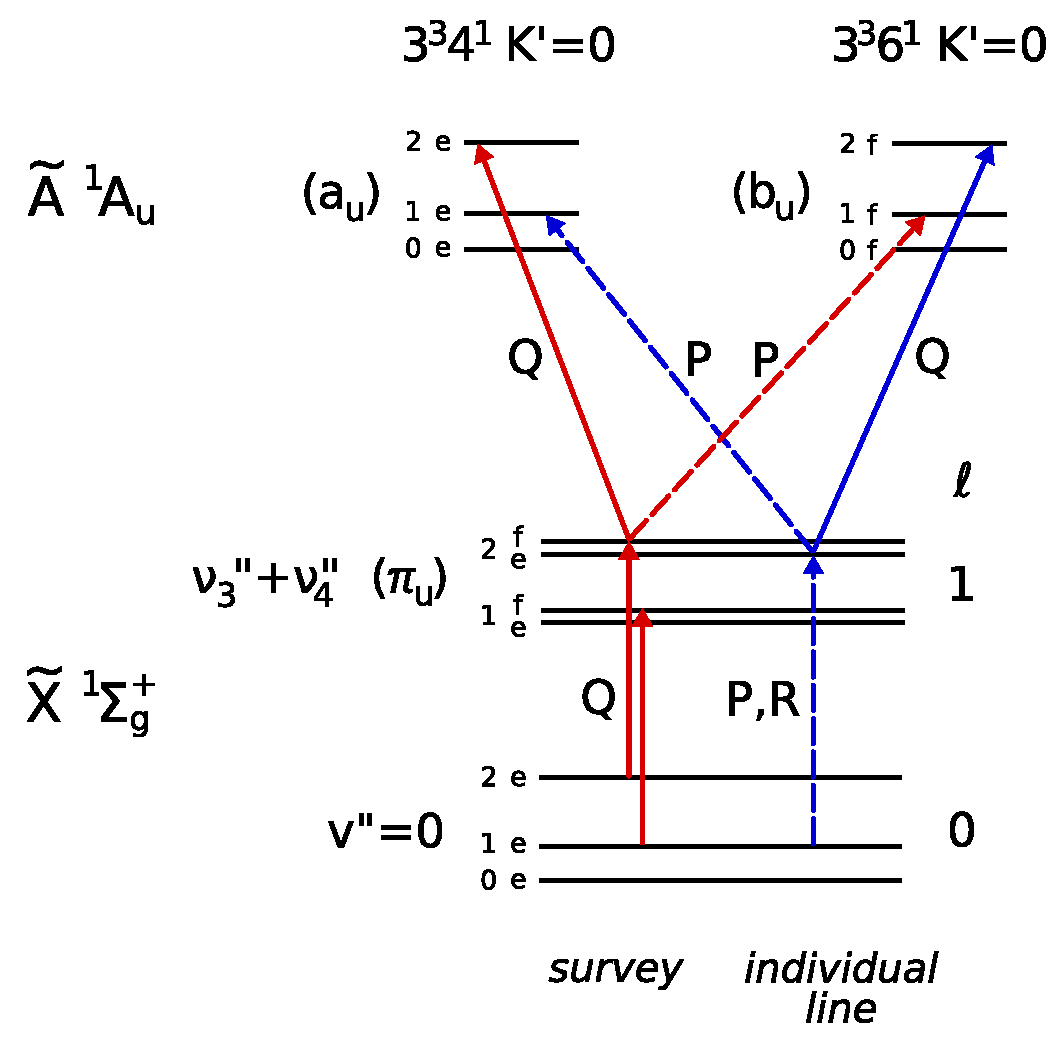
\includegraphics[width=5in]{levels-iruvdr}

  \caption{Schematic diagram of the IR-UV double resonance methods
    used in this study.  In the survey method, the Q(1)-Q(5)
    transitions terminating in the $\nu_3''+\nu_4''$ level of the
    ground state are pumped at a single IR laser energy.  From the
    resulting $f$-symmetry rotational levels, Q-branch transitions in
    the UV are permitted to the $3^34^1$ \Ka{0} sublevel, and P or
    R-branch transitions are permitted to the $3^36^1$ \Ka{0}
    sublevel.  In the individual method, a single P or R-branch
    transition is excited in the ground state.  In this case,
    $e$-symmetry levels of $\nu_3''+\nu_4''$ are excited by the IR
    laser, and the selection rules for P, R vs. Q branches in the UV
    are reversed.}
  \label{fig:levels-iruvdr}
\end{figure}

In the individual method, the IR laser was tuned to individual
transitions in the P or R-branch of the $\nu_3+\nu_4$ level in the
ground electronic state.  Using this strategy, only a single
$e$-symmetry rotational level of $\nu_3''+\nu_4''$ is populated by the
IR laser at a given frequency.  From the intermediate state, only a
single Q-branch transition to the $3^36^1$ \Ka{0} sublevel of the
\astate\ state is permitted in the UV.  The $3^34^1$ \Ka{0} sublevel
of the \astate\ state is accessible through P or R-branch transitions
from the intermediate state, as shown in Figure
\ref{fig:levels-iruvdr}.


Figures \ref{fig:3361-q1}--\ref{fig:3361-q5} show the simultaneously
recorded SEELEM (plotted upward) and LIF (plotted downward) spectra of
the $J'=1-5$ rotational levels of \astate\ $3^36^1$ \Ka{1}, recorded
using the individual method.  The magnitude of the SEELEM signal was
among the highest ever recorded in our laboratory for the acetylene
molecule. The SEELEM:LIF intensity ratio was on the same order of
magnitude as that of the $3^3$ \Ka{1} sublevel, reported previously
\cite{mishra04}. Figures \ref{fig:3361-q1}--\ref{fig:3361-q5} each
contain a magnified view of the SEELEM spectrum, showing a large
number of transitions to long-lived eigenstates over each energy range
scanned by our UV laser.  Unlike previous experiments, each spectrum
in Figures \ref{fig:3361-q1}--\ref{fig:3361-q5} contains eigenstates
having only one value of the rotational quantum number $J$.  Using the
individual double resonance method, the full envelope of metastable
eigenstates drawing intensity from each singlet basis state may be
viewed without overlap from neighboring transitions.

The LIF spectra in Figures \ref{fig:3361-q1}--\ref{fig:3361-q5} are
integrated in two time regions: an early time window
($0.5\tau_s-2\tau_s$, solid trace) and a delayed time window
($10\tau_s-18\tau_s$, dashed trace).  Line splittings are apparent in
the early and delayed LIF spectra of the $J'=1-4$ rotational levels.
The frequency separation of the components in the splittings varies
between 0.06 and 0.2 \rcm.  In the figure, the line with greatest
intensity in the early LIF spectrum is marked with a solid indicator.
Additional lines, appearing with greater intensity in the delayed LIF
spectrum, are marked with dashed indicators.

Differing line intensities in the early vs. delayed LIF spectrum arise
from differences in fluorescence lifetimes among eigenstates.  In the
spectra under consideration, all oscillator strength is provided by a
single, optically bright $S_1$ basis state.  Optically dark basis
states, triplet in character, may mix with the bright state by
spin-orbit interaction, according to the selection rule $\Delta J =
0$.  The fluorescence lifetime of the resultant eigenstates is
inversely proportional to the amount of fractional $S_1$ electronic
character, as detailed in Chapter 4, Section 2.  The eigenstate having
the single greatest amount of fractional $S_1$ character is labeled as
the nominal bright state, and has the shortest lifetime among the
ensemble of mixed eigenstates.  Levels having less fractional $S_1$
character have longer lifetimes and greater intensity in the delayed
LIF spectrum, relative to the early LIF spectrum.  Conequently, for
each spectrum we signify only the single highest-intensity line in the
early LIF channel with a solid marker, indicating its status as the
nominal bright state.

%%%%%%%%%%%%%%%%%%%%%%%%%%%%%%%%%%%%%%%%%%%%%%%%%%%%%%
%%
%% INSERT 3^3 6^1 INDIV FIGURES HERE
%%
%%%%%%%%%%%%%%%%%%%%%%%%%%%%%%%%%%%%%%%%%%%%%%%%%%%%%%

\begin{figure}
  \caption{Simultaneously recorded SEELEM (upper trace) and LIF (lower
    trace) spectra of the $3^36^1$ \Ka{0} sublevel of the \astate\
    state of \ce{C2H2}.  The P(2) line of the \xstate\ $\nu_3'' +
    \nu_4''$ level is used as an intermediate state in the experiment,
    so only the Q(1) line is observed in the upper state, according to
    Figure \ref{fig:levels-iruvdr}.  The LIF spectrum is integrated in
    two time regions: an early time window ($0.5\tau_s-2\tau_s$, solid
    trace) and a delayed time window ($10\tau_s-18\tau_s$, dashed
    trace).  Two additional lines, labeled with dashed markers, are
    observed in the delayed LIF spectrum on either side of the
    nominally singlet eigenstate.}
  \label{fig:3361-q1}
  \centering
  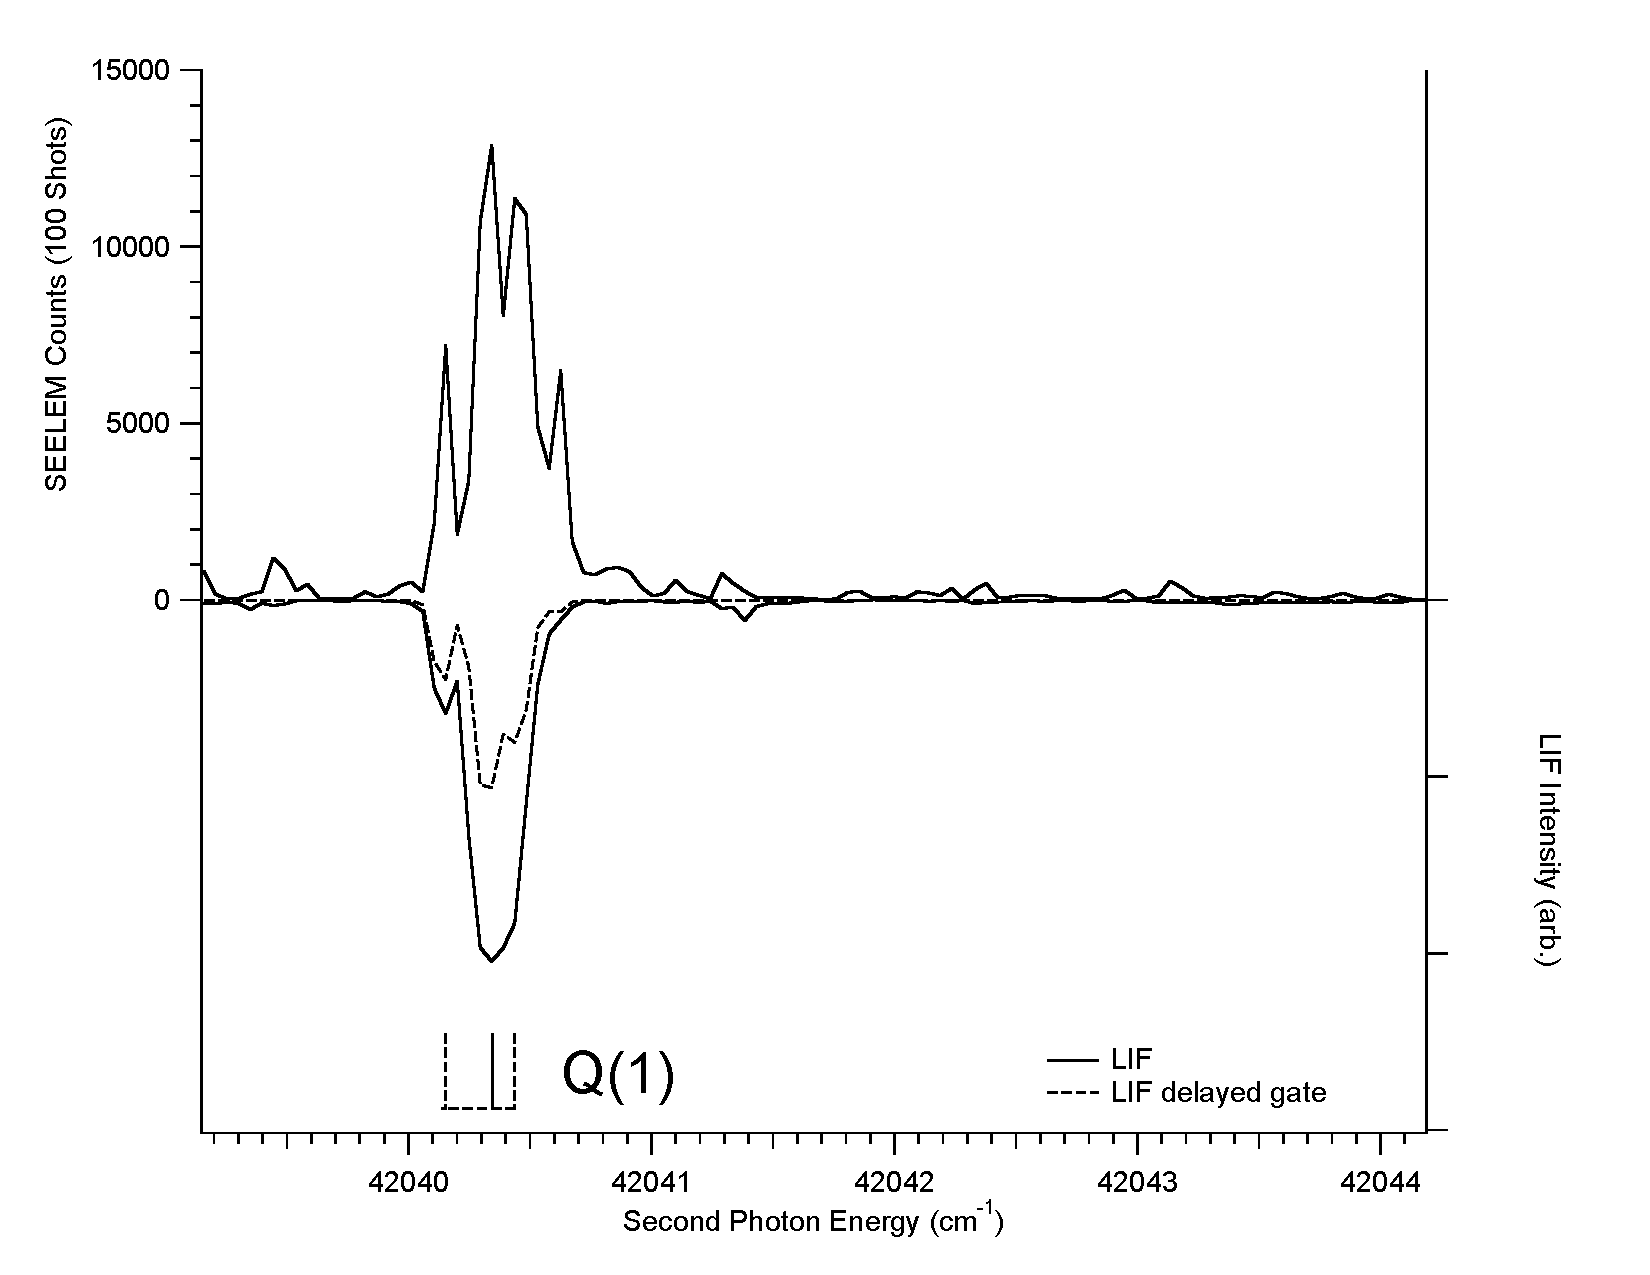
\includegraphics[width=6in]{spectrum-3361-q1-split.pdf}
  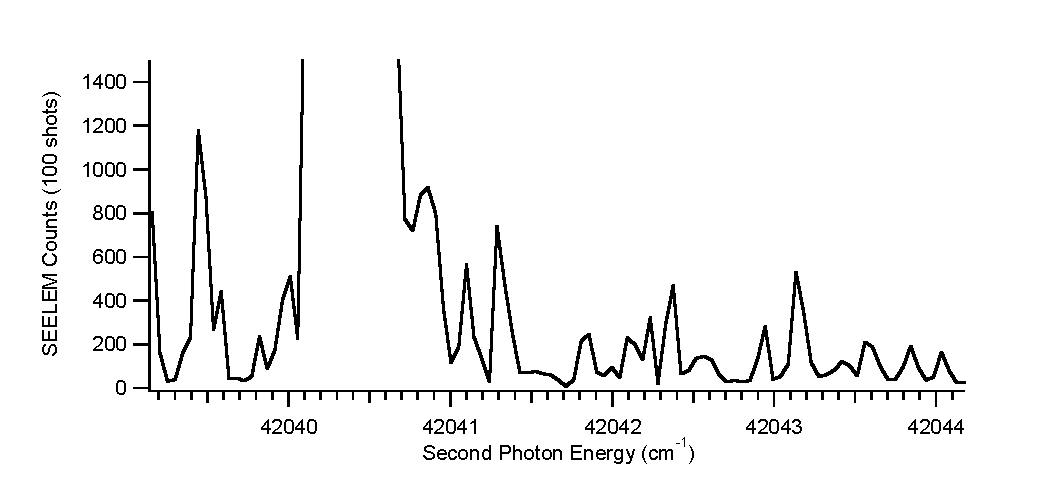
\includegraphics[width=5.5in]{spectrum-3361-q1-zoom.pdf}
\end{figure}

\begin{figure}
  \caption{Simultaneously recorded SEELEM (upper trace) and LIF (lower
    trace) spectra of the $3^36^1$ \Ka{0} sublevel of the \astate\
    state of \ce{C2H2}.  The P(3) line of the \xstate\ $\nu_3'' +
    \nu_4''$ level is used as an intermediate state in the experiment,
    so only the Q(2) line is observed in the upper state, according to
    Figure \ref{fig:levels-iruvdr}.  The LIF spectrum is integrated in
    two time regions: an early time window ($0.5\tau_s-2\tau_s$, solid
    trace) and a delayed time window ($10\tau_s-18\tau_s$, dashed
    trace).  A line splitting of $\sim 2$\rcm\ is observed in the LIF
    spectrum, with the longer-lifetime (nominally triplet) component
    located at higher energy.}
  \label{fig:3361-q2}
  \centering
  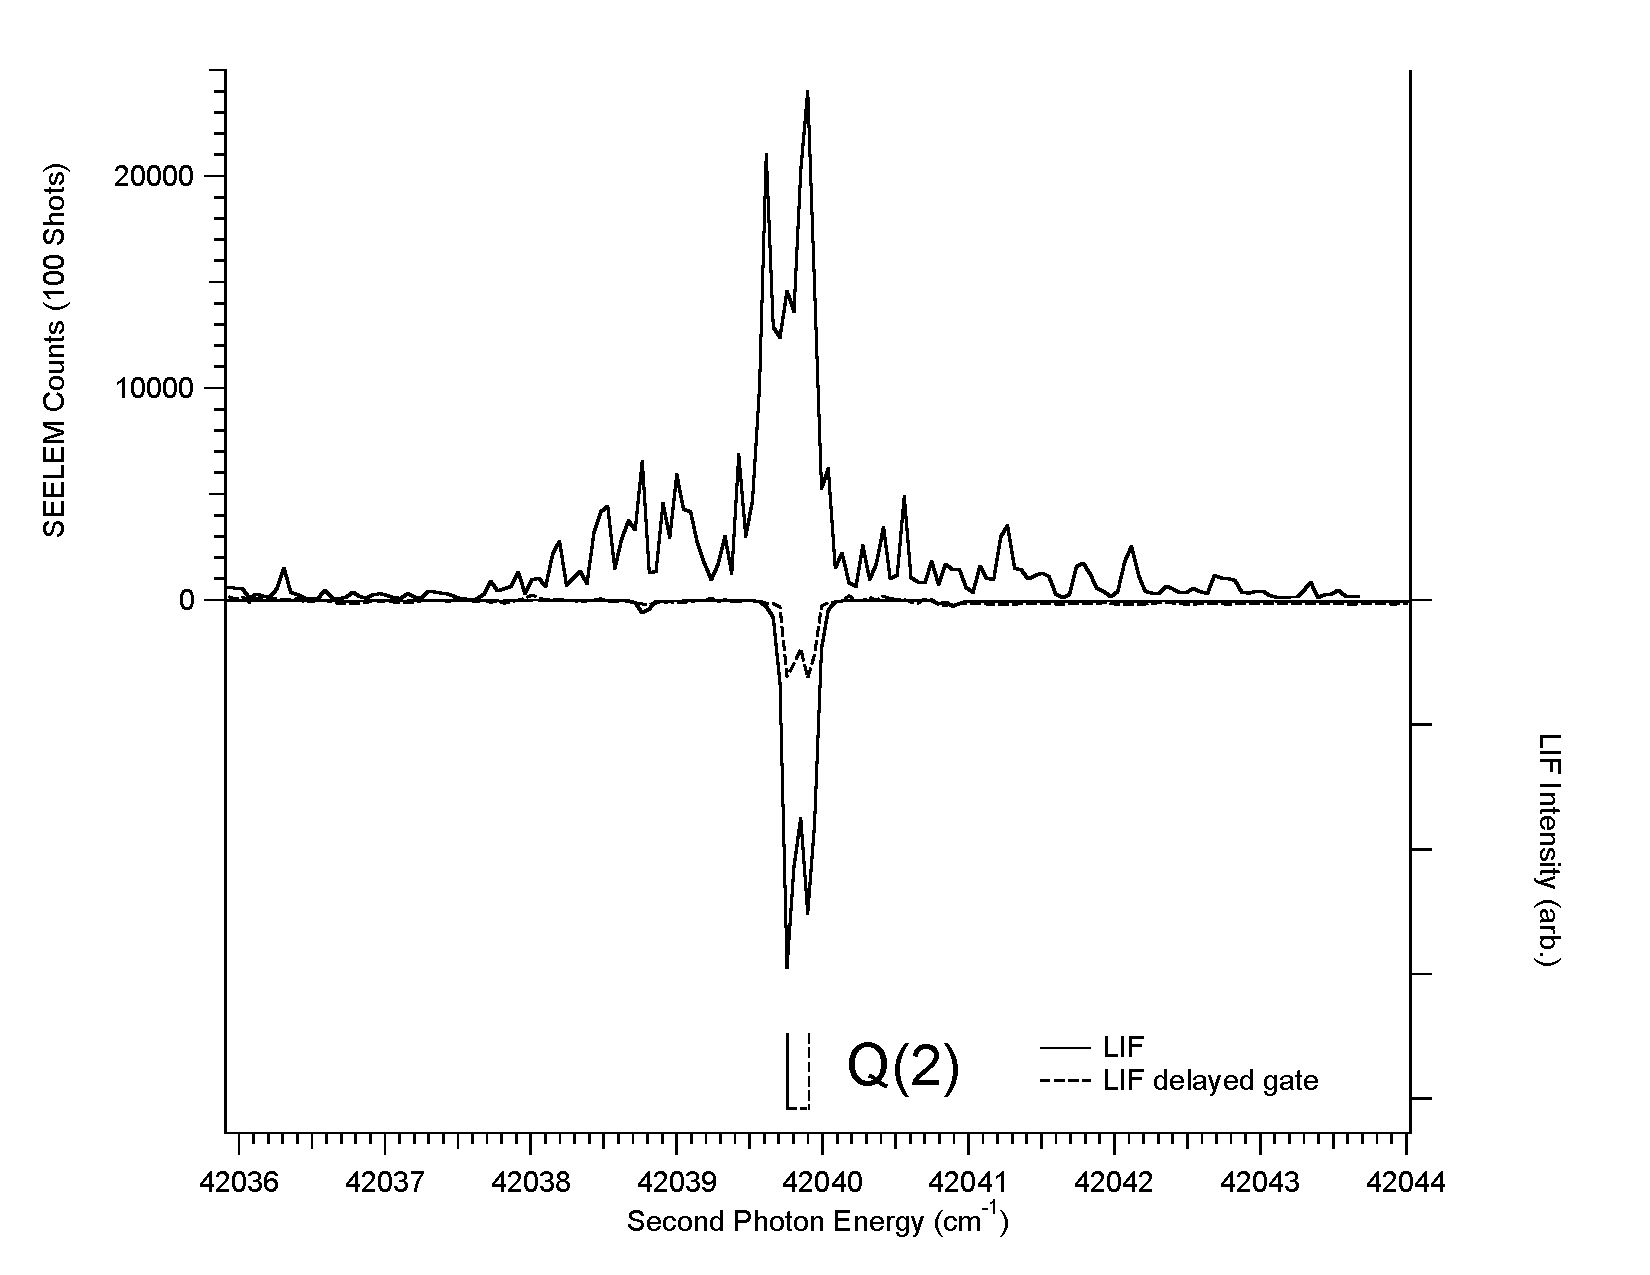
\includegraphics[width=6in]{spectrum-3361-q2-split.pdf}
  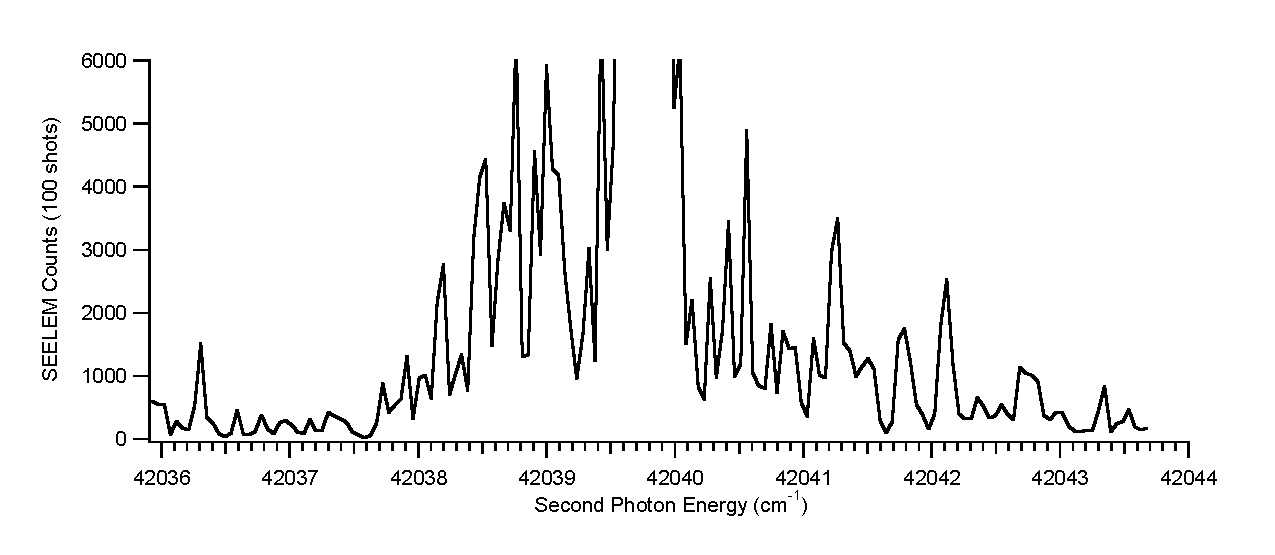
\includegraphics[width=6in]{spectrum-3361-q2-zoom.pdf}
\end{figure}

\begin{figure}
  \caption{Simultaneously recorded SEELEM (upper trace) and LIF (lower
    trace) spectra of the $3^36^1$ \Ka{0} sublevel of the \astate\
    state of \ce{C2H2}.  The P(4) line of the \xstate\ $\nu_3'' +
    \nu_4''$ level is used as an intermediate state in the experiment,
    so only the Q(3) line is observed in the upper state, according to
    Figure \ref{fig:levels-iruvdr}.  The LIF spectrum is integrated in
    two time regions: an early time window ($0.5\tau_s-2\tau_s$, solid
    trace) and a delayed time window ($10\tau_s-18\tau_s$, dashed
    trace).  The transition at 42038.3 \rcm\ has a short lifetime, and
    belongs to an unassigned singlet sublevel.  A small line splitting
    of less than $0.05$\rcm\ is apparent from the shifted peak
    position in the delayed LIF spectrum relative to the early LIF
    spectrum.  The longer-lifetime (nominally triplet) component is
    located to higher energy.}
  \label{fig:3361-q3}
  \centering
  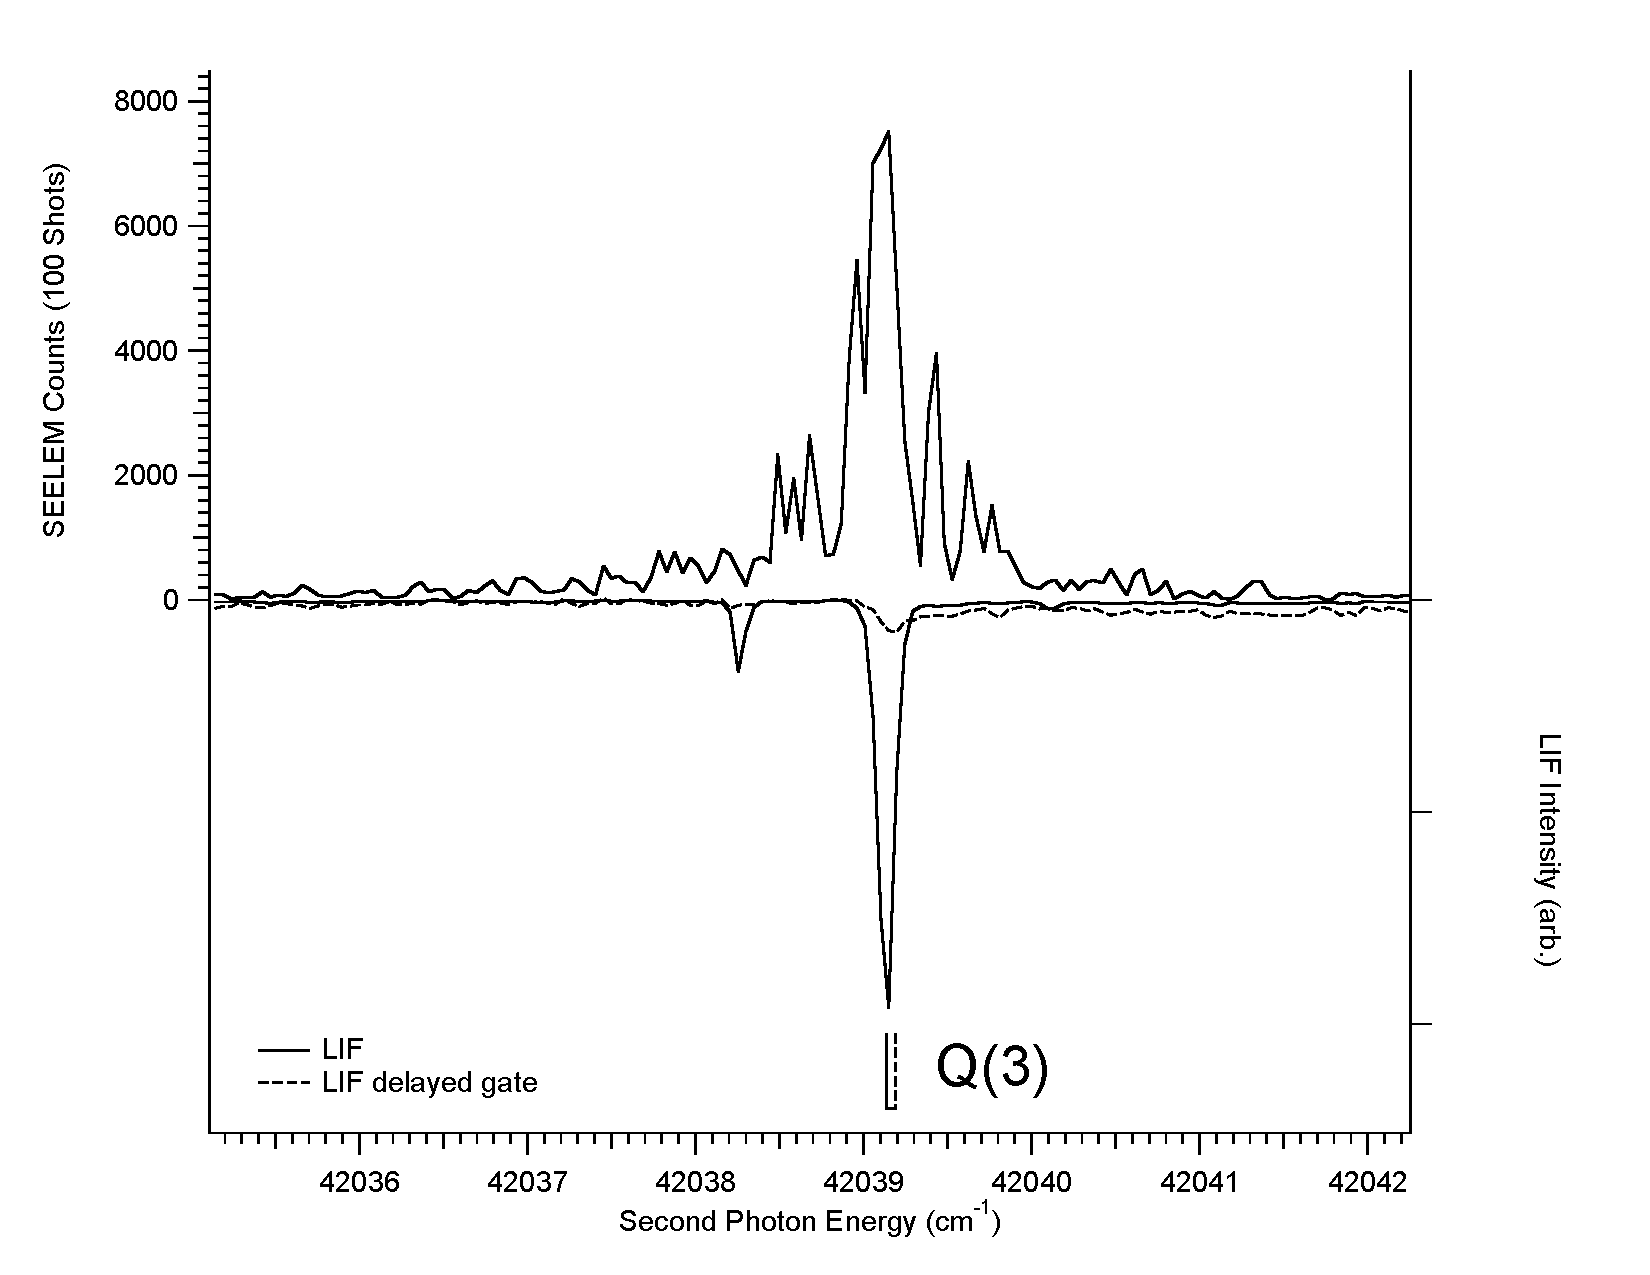
\includegraphics[width=6in]{spectrum-3361-q3-split.pdf}
  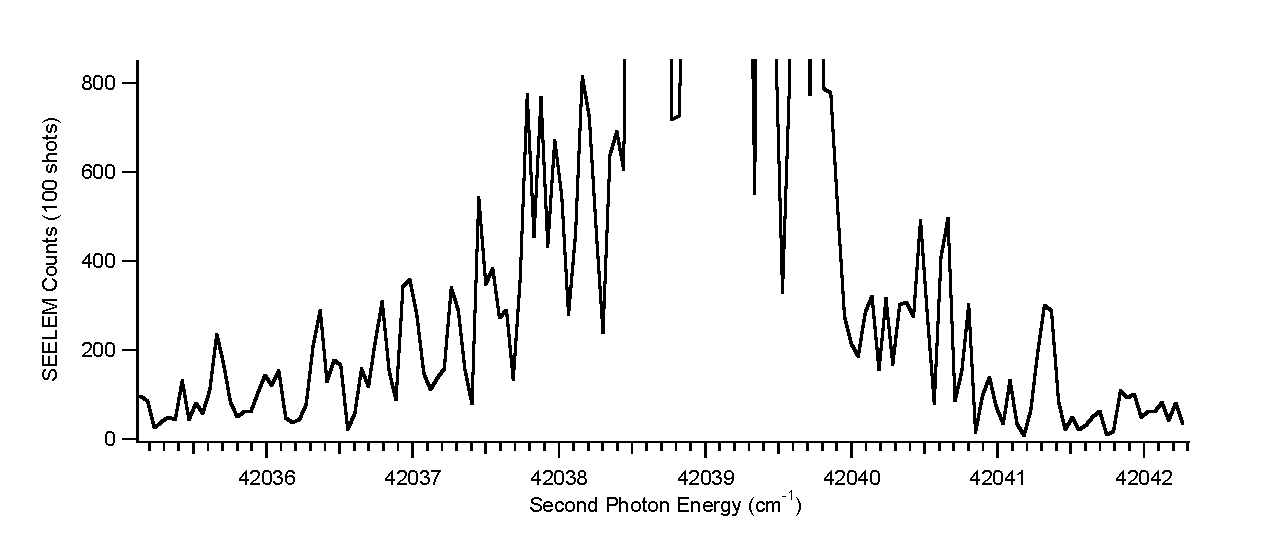
\includegraphics[width=6in]{spectrum-3361-q3-zoom.pdf}
\end{figure}

\begin{figure}
  \caption{Simultaneously recorded SEELEM (upper trace) and LIF (lower
    trace) spectra of the $3^36^1$ \Ka{0} sublevel of the \astate\
    state of \ce{C2H2}.  The R(3) line of the \xstate\ $\nu_3'' +
    \nu_4''$ level is used as an intermediate state in the experiment,
    so only the Q(4) line is observed in the upper state, according to
    Figure \ref{fig:levels-iruvdr}.  The LIF spectrum is integrated in
    two time regions: an early time window ($0.5\tau_s-2\tau_s$, solid
    trace) and a delayed time window ($10\tau_s-18\tau_s$, dashed
    trace).  A line splitting of $\sim0.2$ \rcm\ is observed in the LIF
    spectrum, with the longer-lifetime (nominally triplet) component
    located at higher energy.}
  \label{fig:3361-q4}
  \centering
  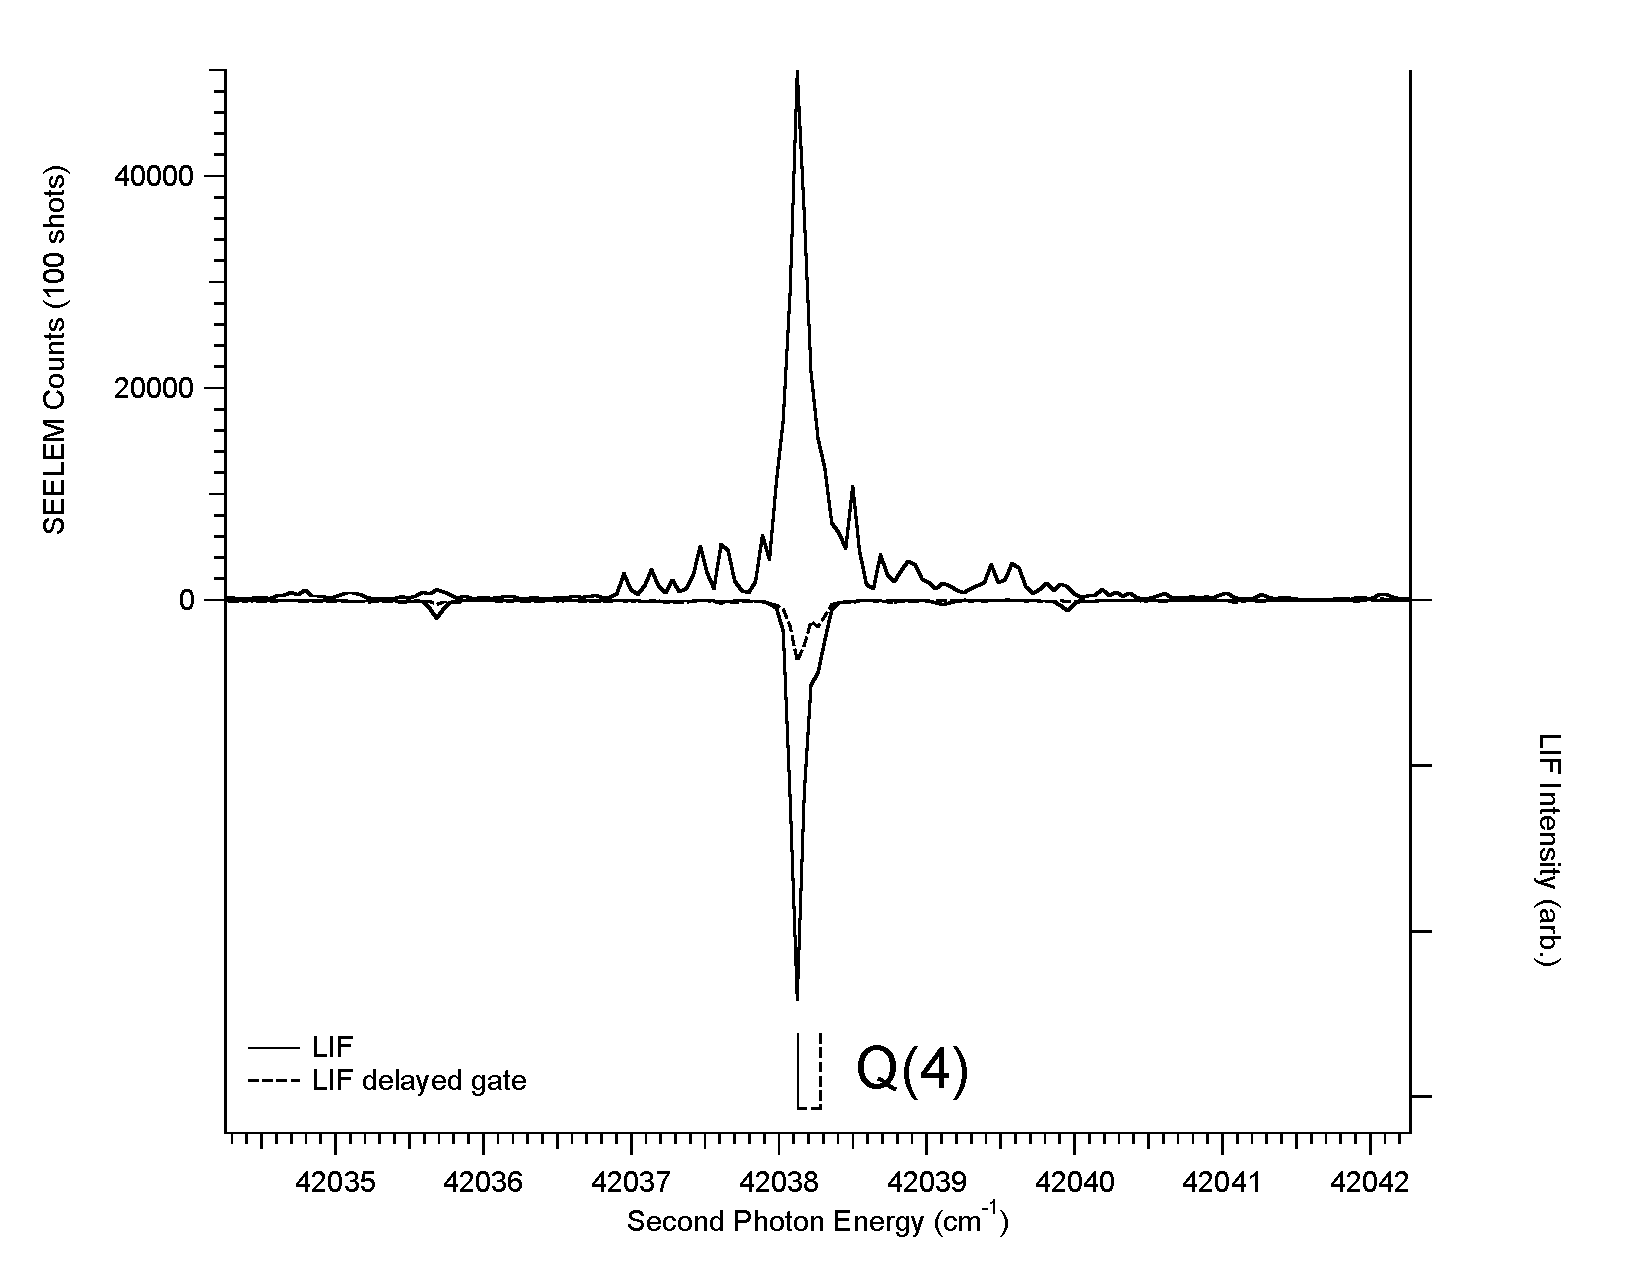
\includegraphics[width=6in]{spectrum-3361-q4-split.pdf}
  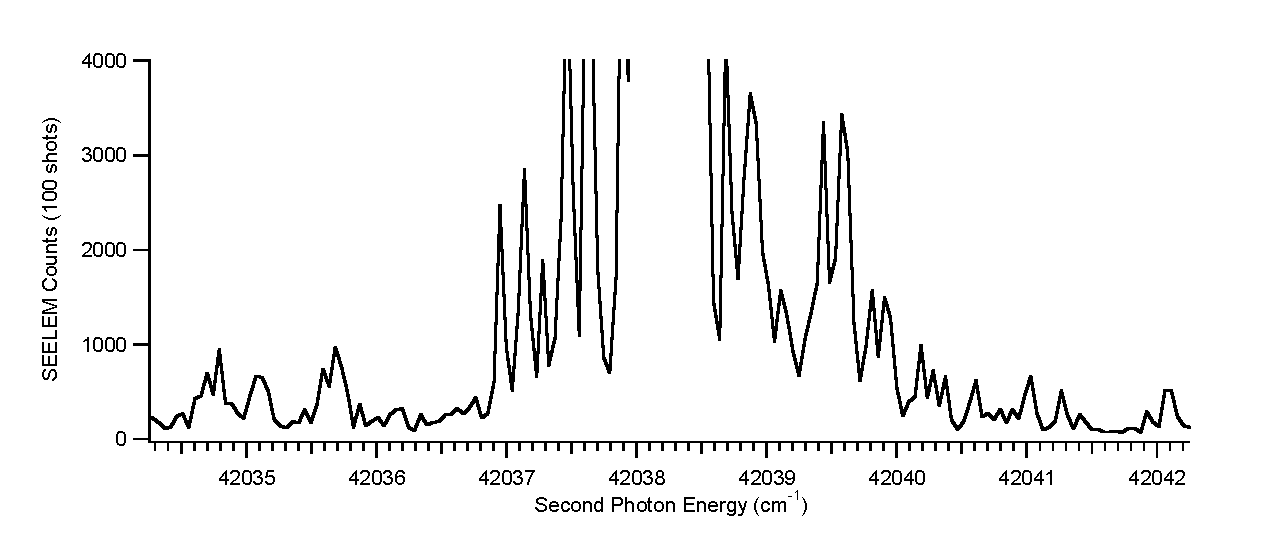
\includegraphics[width=6in]{spectrum-3361-q4-zoom.pdf}
\end{figure}

\begin{figure}
  \caption{Simultaneously recorded SEELEM (upper trace) and LIF (lower
    trace) spectra of the $3^36^1$ \Ka{0} sublevel of the \astate\
    state of \ce{C2H2}.  The R(4) line of the \xstate\ $\nu_3'' +
    \nu_4''$ level is used as an intermediate state in the experiment,
    so only the Q(5) line is observed in the upper state, according to
    Figure \ref{fig:levels-iruvdr}.  The LIF spectrum is integrated in
    two time regions: an early time window ($0.5\tau_s-2\tau_s$, solid
    trace) and a delayed time window ($10\tau_s-18\tau_s$, dashed
    trace).  No line splittings are observed in the LIF spectrum.}
  \label{fig:3361-q5}
  \centering
  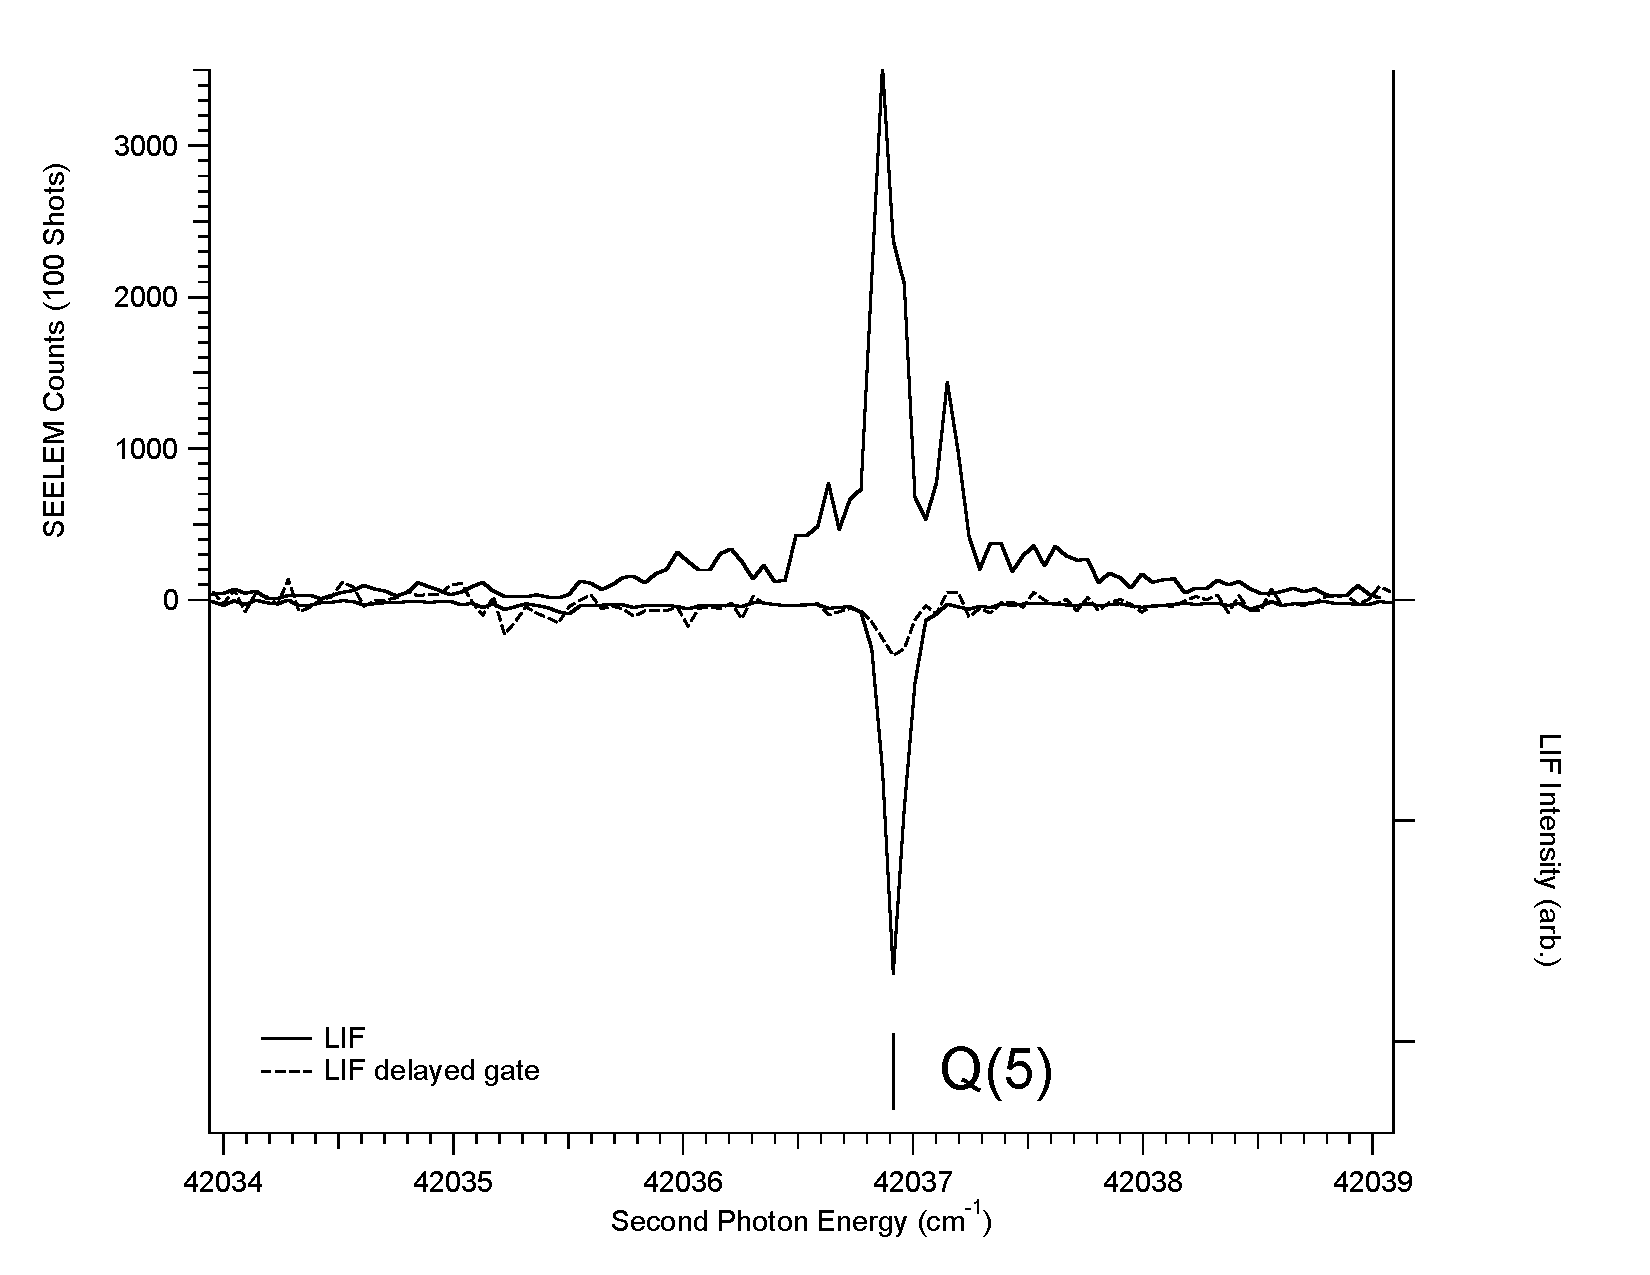
\includegraphics[width=6in]{spectrum-3361-q5-split.pdf}
  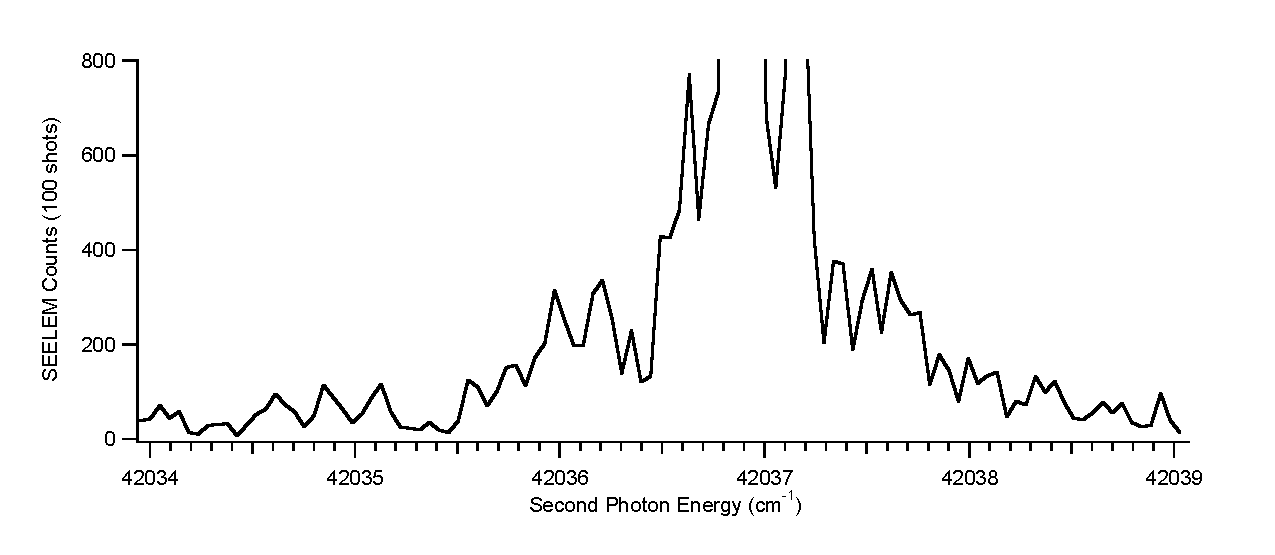
\includegraphics[width=6in]{spectrum-3361-q5-zoom.pdf}
\end{figure}

%%%%%%%%%%%%%%%%%%%%%%%%%%%%%%%%%%%%%%%%%%%%%%%%%%%%%%
%%
%% END OF 3^3 6^1 INDIV FIGURES
%%
%%%%%%%%%%%%%%%%%%%%%%%%%%%%%%%%%%%%%%%%%%%%%%%%%%%%%%











The spectrum of the $J'=0$ rotational level of $3^36^1$ \Ka{0} cannot
be recorded using the individual double resonance method, since only
Q-branch transitions appear in the UV spectrum.  Instead, the spectrum
of $3^36^1$ \Ka{0} was recorded in the region of the P(1) transition
by the survey method, using two relative polarization geometries for
the IR and UV laser beams.  When the polarization of the collinear IR
and UV beams is aligned in a perpedicular geometry, the P(1)
transition is permitted in the UV.  The two-step excitation proceeds
according to the following rules.  Hyperfine levels in the
intermediate state having $M_J=1$ are populated via $\Delta M_J=0$
transitions in the first excitation step.  In the second excitation
step, when the UV laser beam is perpedicularly polarized to the IR
beam, $\Delta M_J = \pm 1$ transitions are permitted to the upper
state $J'=0$ rotational level, which has only one hyperfine component,
$M_J=0$.  Figure \ref{fig:levels-polarization} illustrates the
permitted transitions among hyperfine levels with a series of solid
arrows.  When the collinear IR and UV laser beams have a parallel
polarization, the selection rules for $\Delta M_J$ do not allow for
any transitions terminating in the upper state $J'=0$ rotational
level.  Since the IR and UV beams have identical polarization, the
value of $\Delta M_J$ must be identical in the IR and UV excitation
steps.  A value of $\Delta M_J = + 1$ or $\Delta M_J = - 1$ in both
steps does not accomodate transitions terminating in the $J'=0$
rotational level of the excited state.  A value of $\Delta M_J = 0$
for both steps could possibly terminate in the $J'=0$ rotational level
of the excited state, but such a transition is forbidden in the first
step, according to the selection rule that $M_J=0 \nleftrightarrow
M_J=0$ for $\Delta J = 0$ (Q-branch) tansitions \cite{herzberg66}.
The forbidden transition is illustrated with dashed arrows in Figure
\ref{fig:levels-polarization}.  According to the selection rules for
$\Delta M_J$, the transition to $J'=0$ in the excited state is
forbidden for parallel laser polarization.

%%%%%%%%%%%%%%%%%%%%%%%%%%%%%%%%%%%%%%%%%%%%%%%%%%%%%%%
%%
%% INSERT POLARIZATION DIAGRAM
%%
%%%%%%%%%%%%%%%%%%%%%%%%%%%%%%%%%%%%%%%%%%%%%%%%%%%%%%%

\begin{figure}
  \caption{Diagram of transitions among hyperfine levels terminating
    in the $J'=0$ rotational level of $3^36^1$ \Ka{0}.  When the IR
    and UV lasers are polarized in a perpendicular geometry,
    transitions terminating in the $J'=0$ rotational level of the
    excited state are permitted according to the selection rules
    $\Delta M_J = 0$ (first step), $\Delta M_J = \pm 1$ (second step).
    When the IR and UV lasers are polarized in a parallel geometry,
    transitions terminating in the $J'=0$ rotational level of the
    excited state are forbidden according to the selection rule $M_J =
    0 \nleftrightarrow M_J = 0$ when $\Delta J = 0$.}
  \label{fig:levels-polarization}

  \centering
  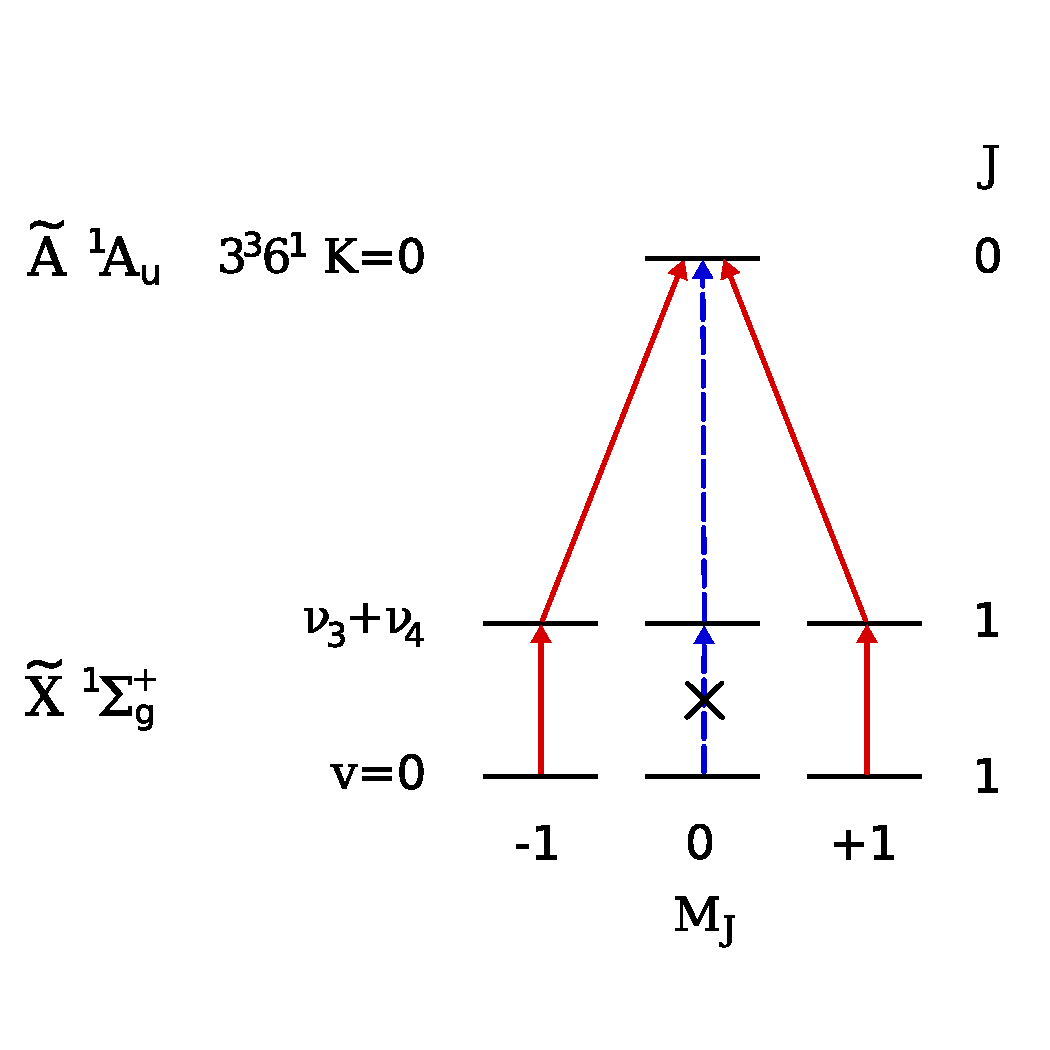
\includegraphics[width=5in]{levels-polarization.pdf}
\end{figure}

%%%%%%%%%%%%%%%%%%%%%%%%%%%%%%%%%%%%%%%%%%%%%%%%%%%%%%
%%
%% END POLARIZATION DIAGRAM
%%
%%%%%%%%%%%%%%%%%%%%%%%%%%%%%%%%%%%%%%%%%%%%%%%%%%%%%%


The simultaneously recorded SEELEM/LIF spectra of $3^36^1$ \Ka{0} in
the region of the P(1) transition are shown in Figure
\ref{fig:3361-p1-polarization} for perpendicular (solid trace) and
parallel (dashed trace) laser polarization.  Since the transition to
$J'=0$ is forbidden in the parallel geometry, the dashed trace serves
as a null spectrum in this region.  At UV frequencies between 42036.0
and 42041.3 \rcm, essentially all peaks in the SEELEM spectrum are due
to intensity borrowing from the $J'=0$ level of $3^36^1$ \Ka{0}.  This
particular region is shown with more detail in Figure
\ref{fig:3361-p1}.  The delayed LIF spectrum is also included as a
dashed trace in this figure.  A line splitting is resolved in the
delayed LIF, with the long-lifetime component lying to higher
frequency.

%%%%%%%%%%%%%%%%%%%%%%%%%%%%%%%%%%%%%%%%%%%%%%%%%%%%%%
%%
%% INSERT 3^3 6^1 POLARIZATION FIGURES HERE
%%
%%%%%%%%%%%%%%%%%%%%%%%%%%%%%%%%%%%%%%%%%%%%%%%%%%%%%%

\begin{figure}
  \caption{Simultaneously recorded SEELEM (upper trace) and LIF (lower
    trace) spectra of the $3^36^1$ \Ka{0} sublevel of the \astate\
    state of \ce{C2H2}.  The Q-branch of the \xstate\ $\nu_3'' +
    \nu_4''$ level is used as an intermediate transition in the
    experiment, so all P- and R-branch lines are observed in the upper
    state, according to Figure \ref{fig:levels-iruvdr}.  The P(1)
    transition to the upper state is forbidden in a parallel IR-UV
    laser polarization geometry.  A spectrum taken with this laser
    geometry is shown with a dashed line.}
  \label{fig:3361-p1-polarization}
  \centering
  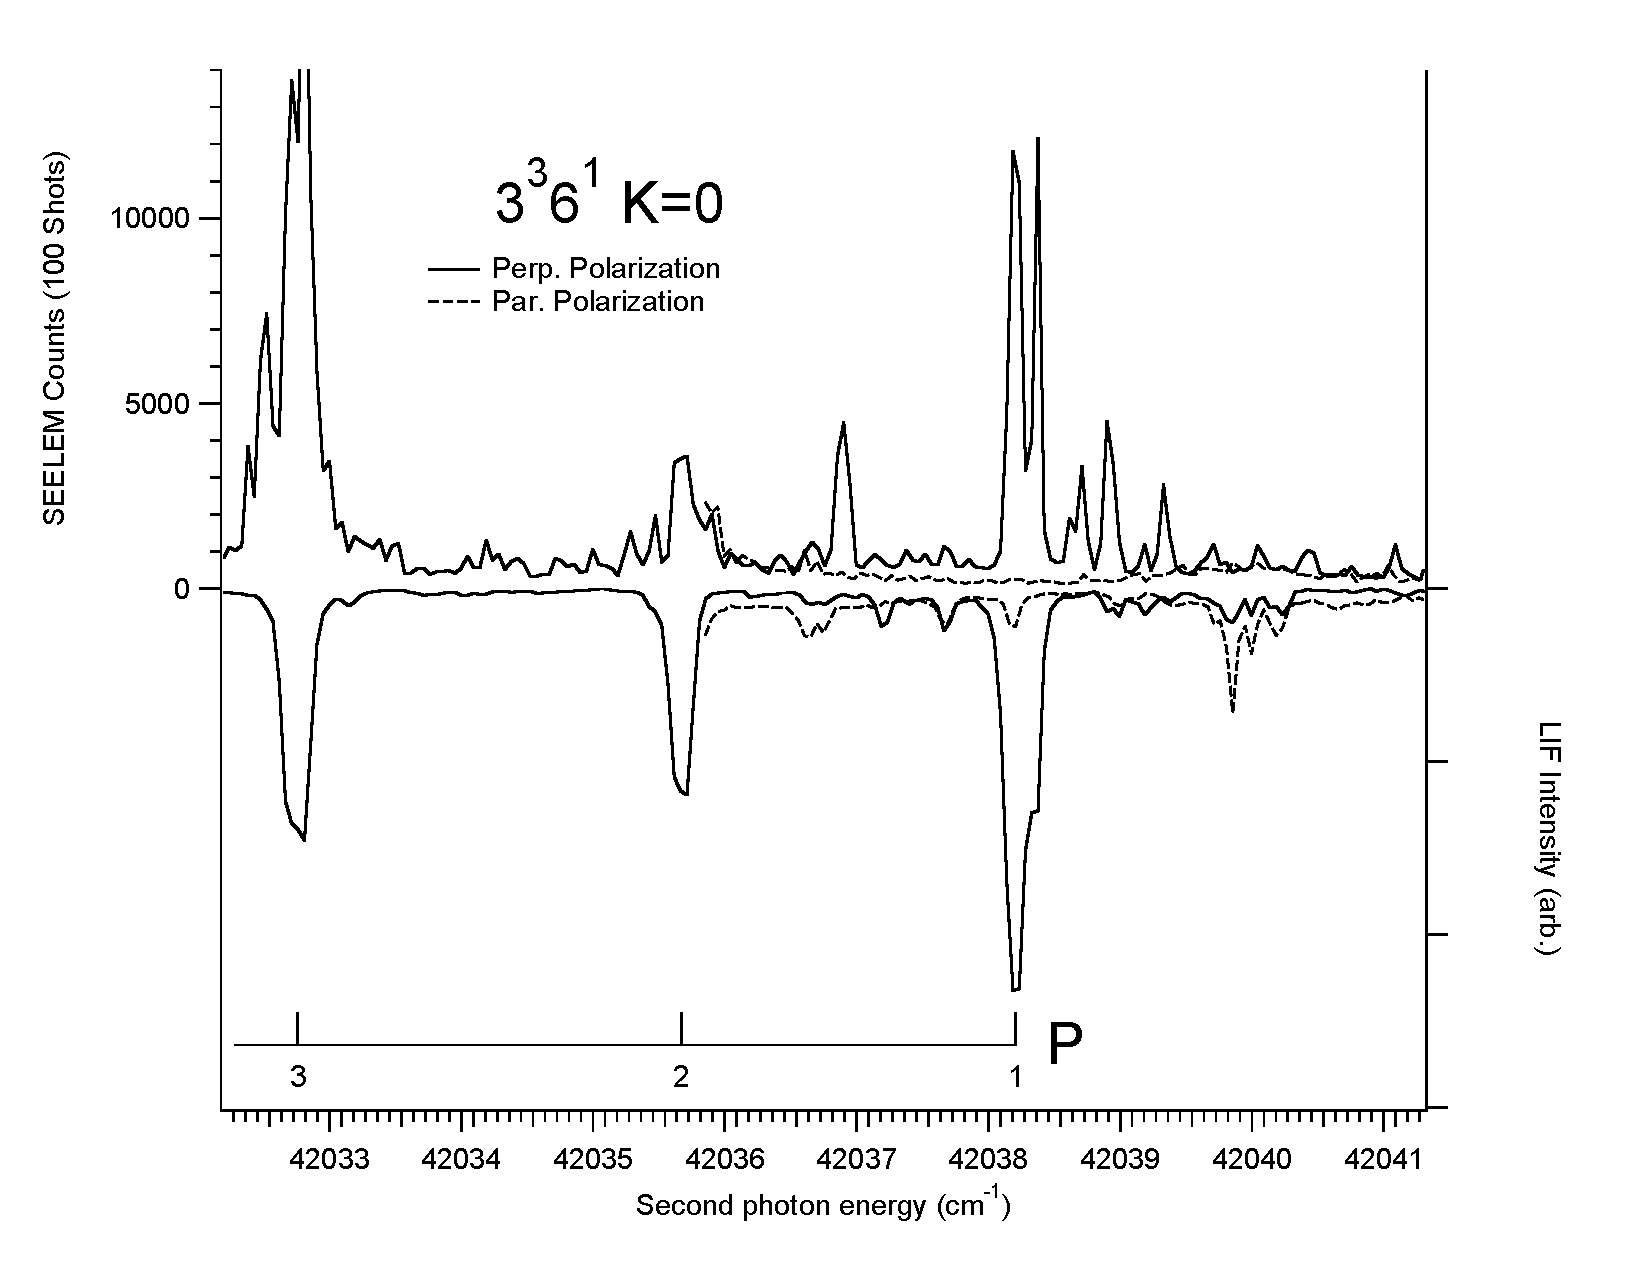
\includegraphics[width=7.3in,angle=90]{spectrum-3361-p1.pdf}
\end{figure}


\begin{figure}
  \caption{Simultaneously recorded SEELEM (upper trace) and LIF (lower
    trace) spectra of the $3^36^1$ \Ka{0} sublevel of the \astate\
    state of \ce{C2H2}.  The Q-branch of the \xstate\ $\nu_3'' +
    \nu_4''$ level is used as an intermediate transition in the
    experiment, so all P- and R-branch lines are observed in the upper
    state, according to Figure \ref{fig:levels-iruvdr}.  The LIF
    spectrum is integrated in two time regions: an early time window
    ($0.5\tau_s-2\tau_s$, solid trace) and a delayed time window
    ($10\tau_s-18\tau_s$, dashed trace).  A line splitting of $\sim
    2$\rcm\ is observed in the LIF spectrum, with the longer-lifetime
    (nominally triplet) component located at higher energy. \TODO{Fix
      energy axis.}}
  \label{fig:3361-p1}
  \centering
  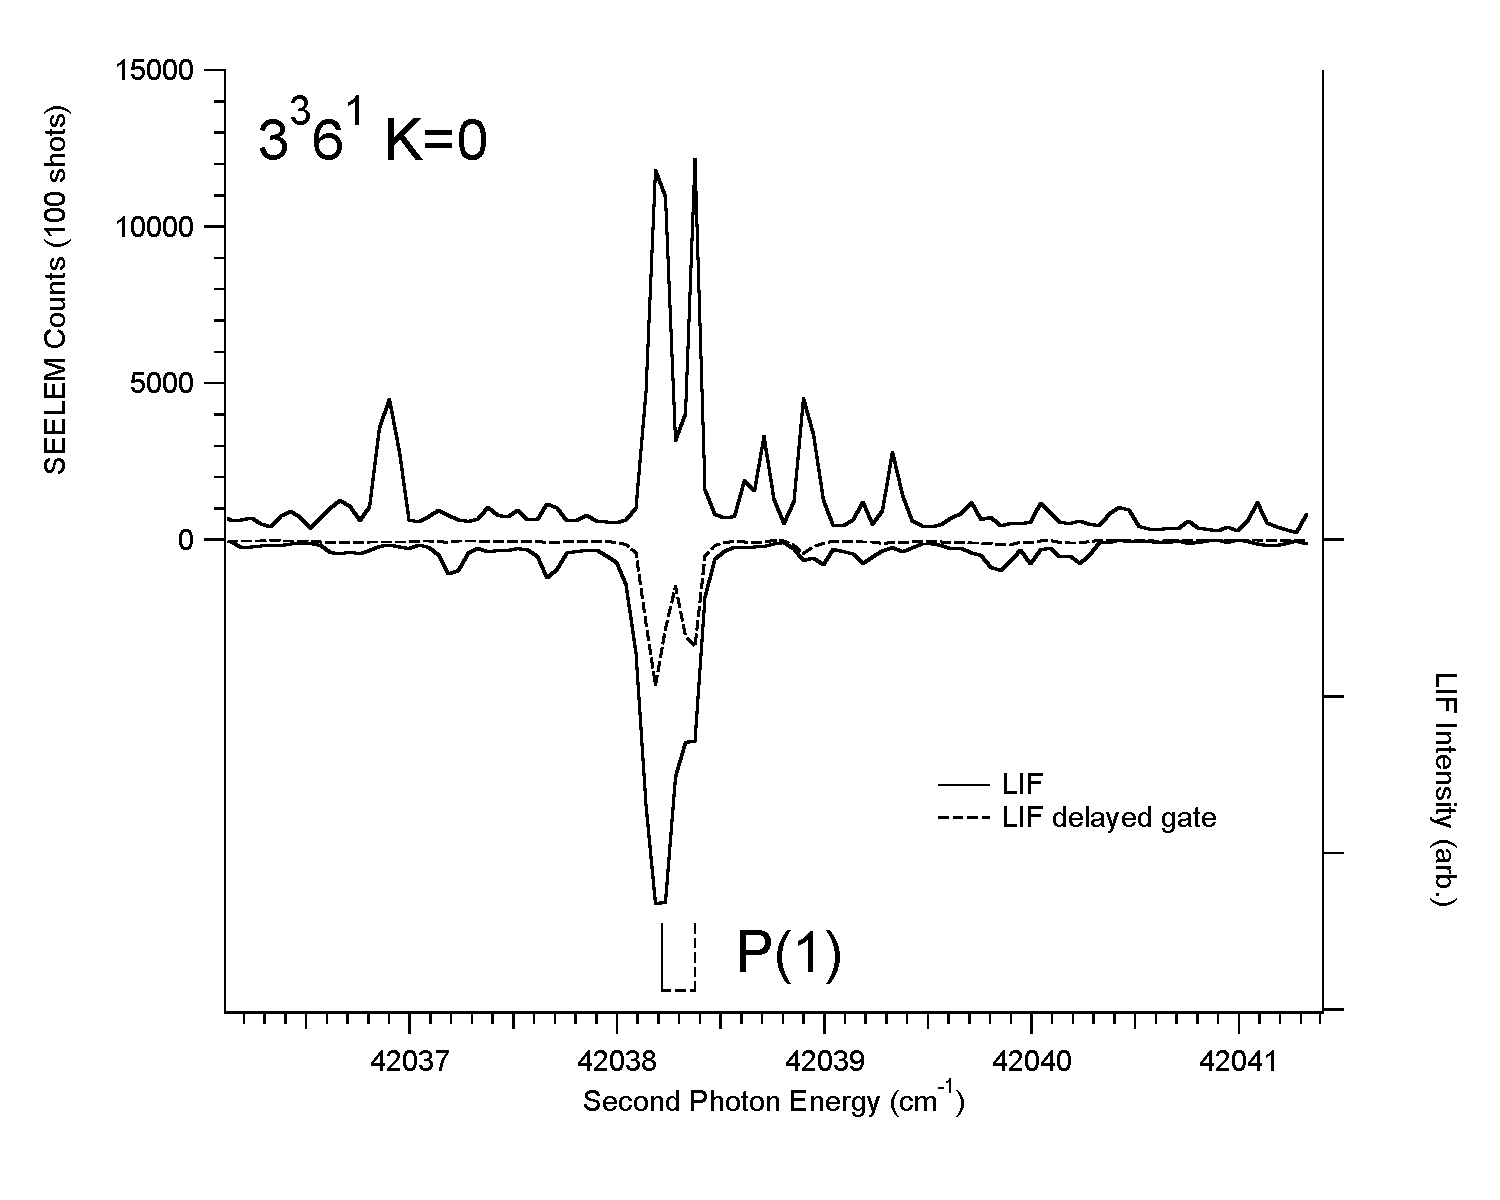
\includegraphics[width=5.8in]{spectrum-3361-p1-split}
  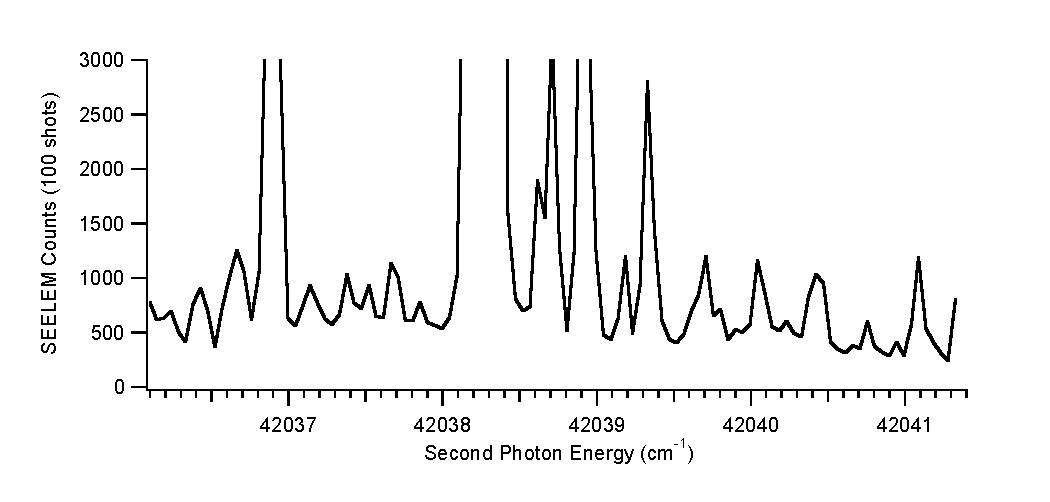
\includegraphics[width=6in]{spectrum-3361-p1-zoom}
\end{figure}

%%%%%%%%%%%%%%%%%%%%%%%%%%%%%%%%%%%%%%%%%%%%%%%%%%%%%%
%%
%% END OF 3^3 6^1 POLARIZATION FIGURES
%%
%%%%%%%%%%%%%%%%%%%%%%%%%%%%%%%%%%%%%%%%%%%%%%%%%%%%%%
































The SEELEM/LIF spectrum of $3^34^1$ \Ka{0}, recorded via the survey
method, is shown in Figure \ref{fig:survey-3341}.  The LIF spectrum is
integrated in both early ($0.5\tau_s-2\tau_s$, solid trace) and
delayed ($10\tau_s-18\tau_s$, dashed trace) time windows.  Due to
saturation of the photomultiplier tube at early time intervals, the
early LIF spectrum shown in the figure was recorded and calibrated in
a separate scan.  The delayed LIF spectrum and the SEELEM spectrum
were acquired simultaneously.  The integrated SEELEM:LIF intensity
ratio is observed to be on the same order of magnitude as that of the
$3^36^1$ \Ka{0} level.

Line splittings appear in the delayed LIF spectrum of every transition
to the $3^34^1$ \Ka{0} sublevel.  The splittings span a frequency
range of $0.06-0.3$ \rcm.  The average frequency between components
having the same $J'$ is slightly larger than that of $3^36^1$ \Ka{0},
and in general they are more pronounced in the early LIF spectrum.
Presumably the line splittings in $3^34^1$ \Ka{0} were too small to be
detected by Mizoguchi and coworkers, who recorded and assigned the LIF
spectrum of this level previously, and cite a UV laser resolution of
0.1 \rcm \cite{mizoguchi00}.  The line splittings reported in that
reference, observed in another sublevel, are an order of magnitude
larger than those observed in this spectrum.

The line splitting in Q(1) could not be assigned directly from the
survey spectrum, since the long-lifetime component appears at a
frequency halfway between the Q(1) and Q(2) transitions.  To assign
the long-lifetime component, the spectrum of the P(2) transition in
$3^34^1$ \Ka{0} was recorded using the individual method.  The
$\nu_3''+\nu_4''$ intermediate level was accessed via the P(3)
transition from the ground state.  This spectrum is shown in Figure
\ref{fig:3341-p2}.  A large line splitting of -0.25 \rcm\ is observed
in the LIF spectrum, confirming the assignment of the long-lifetime
component as $J'=1$.

%%%%%%%%%%%%%%%%%%%%%%%%%%%%%%%%%%%%%%%%%%%%%%%%%%%%%%
%%
%% INSERT 3^3 4^1 FIGURES HERE
%%
%%%%%%%%%%%%%%%%%%%%%%%%%%%%%%%%%%%%%%%%%%%%%%%%%%%%%%

\begin{figure}
  \caption{Simultaneously recorded SEELEM (upper trace) and LIF (lower
    trace) spectra of the $3^34^1$ \Ka{0} sublevel of the \astate\
    state of \ce{C2H2}.  The Q-branch of the \xstate\ $\nu_3'' +
    \nu_4''$ level is used as an intermediate transition in the
    experiment, so all Q-branch lines are observed in the upper state,
    according to Figure \ref{fig:levels-iruvdr}.  The LIF spectrum is
    integrated in two time regions: an early time window
    ($0.5\tau_s-2\tau_s$, solid trace) and a delayed time window
    ($10\tau_s-18\tau_s$, dashed trace).  Line splittings ranging from
    0.06 to 0.3 \rcm\ are observed in the delayed LIF spectrum of all
    rotational lines.  With one exception, the longer-lifetime
    (nominally triplet) components are located to lower energy.}
  \label{fig:survey-3341}
  \centering
  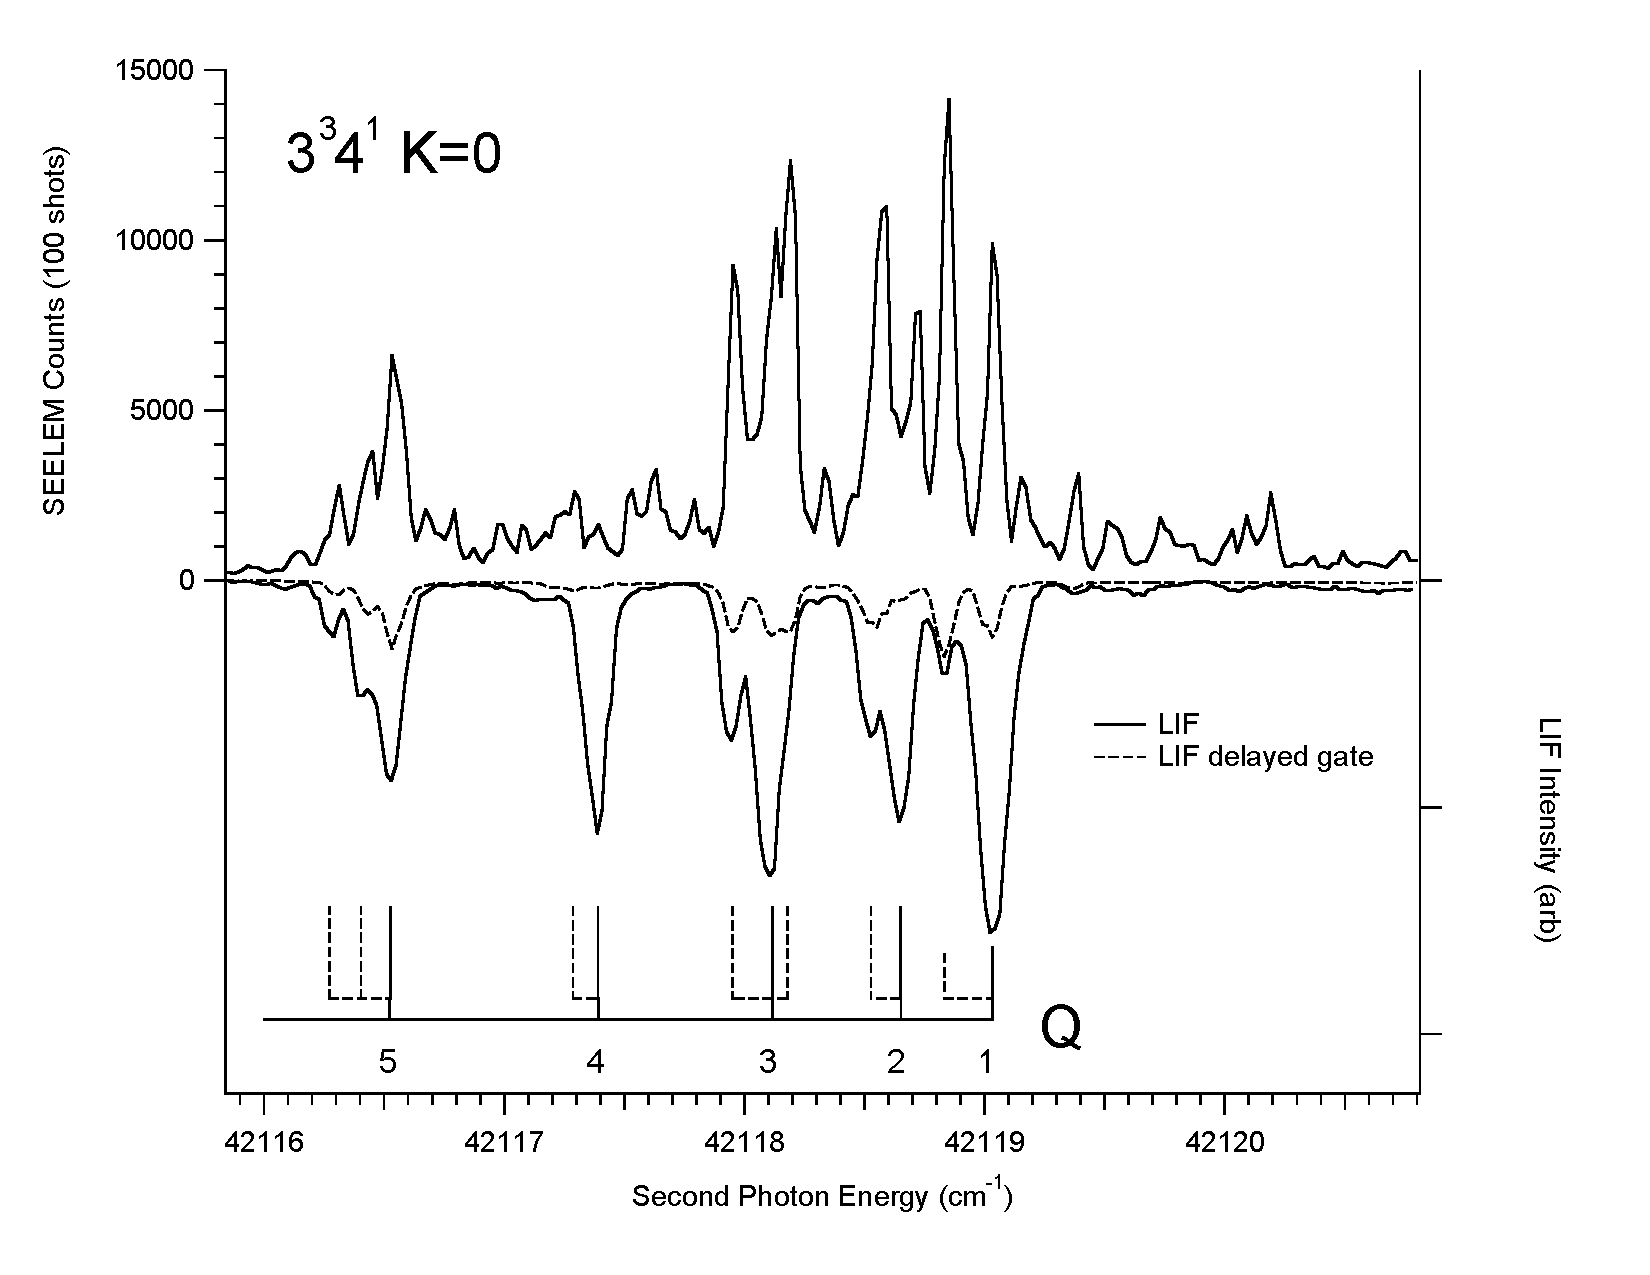
\includegraphics[width=7in,angle=90]{spectrum-3341-q5q1-split.pdf}
\end{figure}

\begin{figure}
  \caption{Simultaneously recorded SEELEM (upper trace) and LIF (lower
    trace) spectra of the $3^34^1$ \Ka{0} sublevel of the \astate\
    state of \ce{C2H2}.  The P(3) line of the \xstate\ $\nu_3'' +
    \nu_4''$ level is used as an intermediate state in the experiment,
    so only the P(2) line is observed in the upper state, according to
    Figure \ref{fig:levels-iruvdr}.  The LIF spectrum is integrated in
    two time regions: an early time window ($0.5\tau_s-2\tau_s$, solid
    trace) and a delayed time window ($10\tau_s-18\tau_s$, dashed
    trace).  A large line splitting of -0.25 \rcm\ is observed in the
    delayed fluorescence, confirming the assignment of the low-energy
    component as $J'=1$.  \TODO{Calibration.}}
  \label{fig:3341-p2}
  \centering
  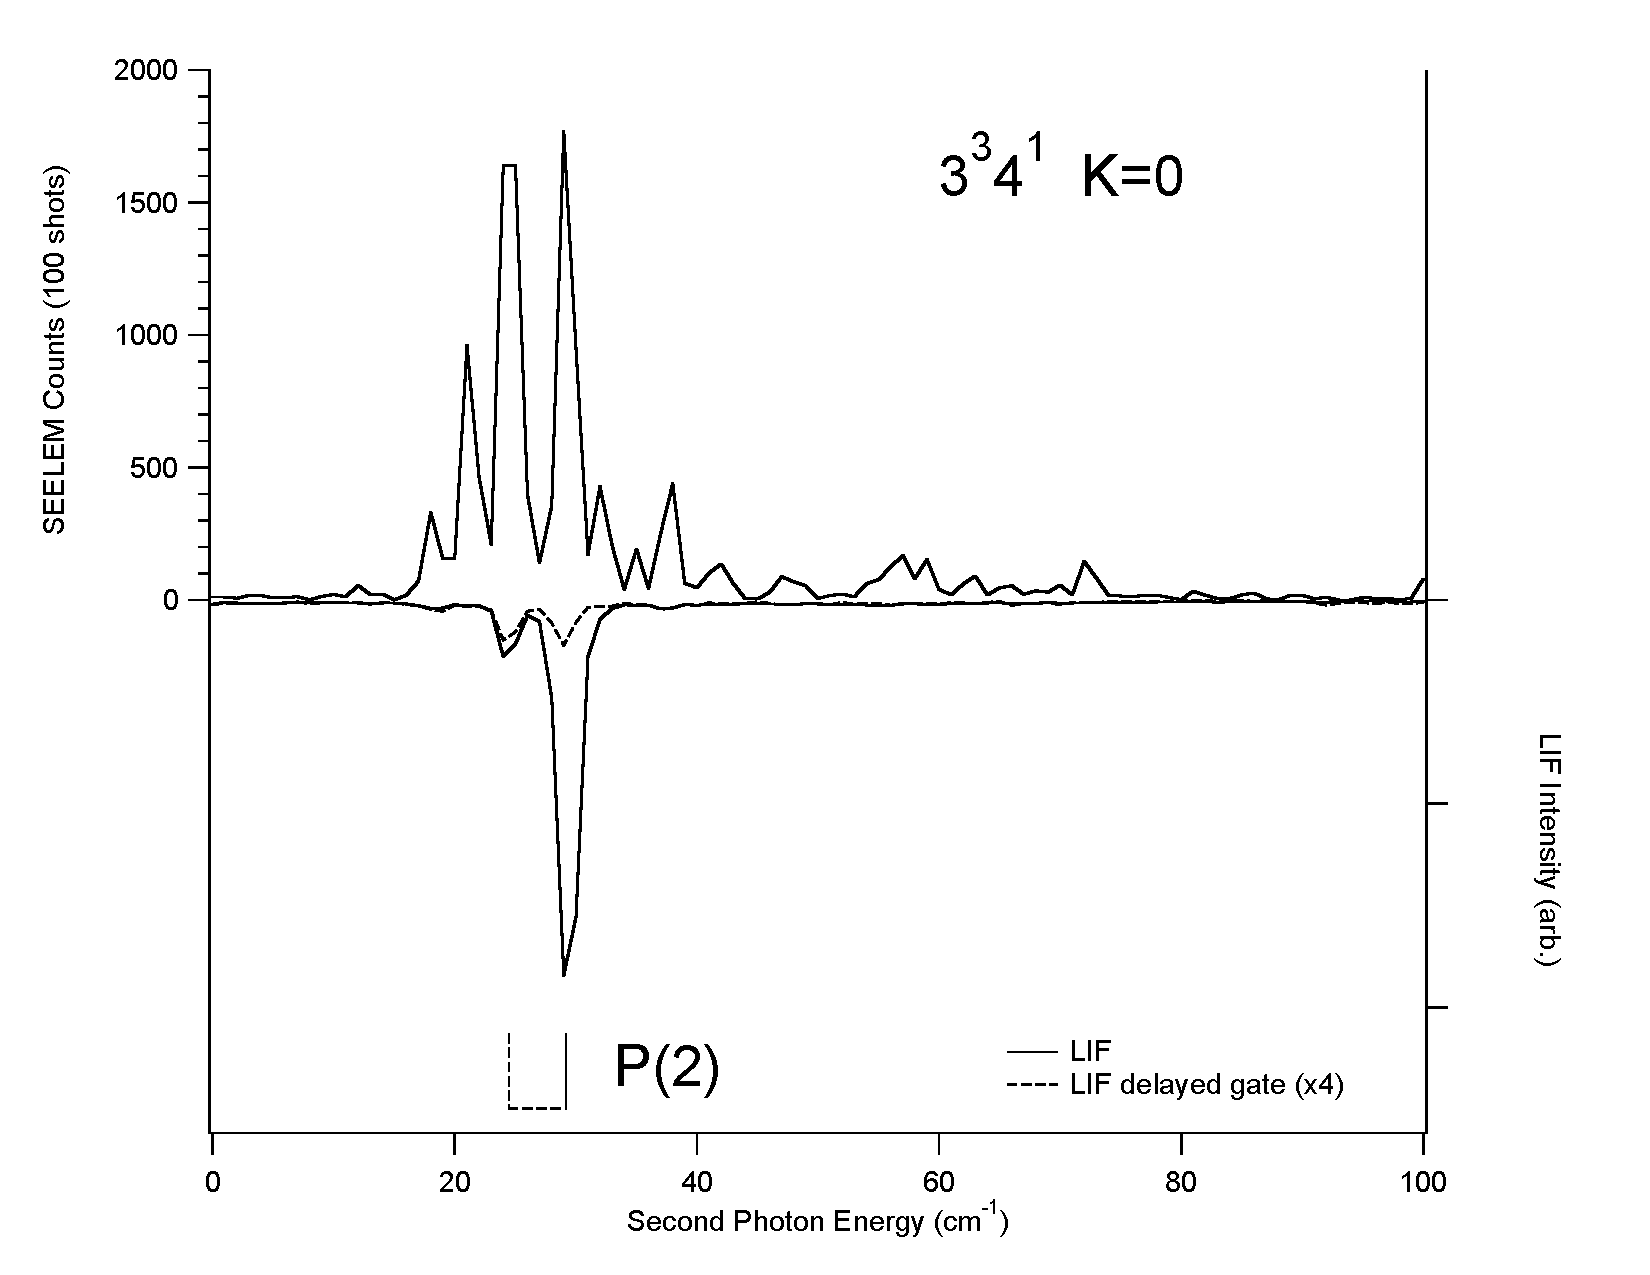
\includegraphics[width=6in]{spectrum-3341-p2-split.pdf}
\end{figure}

%%%%%%%%%%%%%%%%%%%%%%%%%%%%%%%%%%%%%%%%%%%%%%%%%%%%%%
%%
%% END OF 3^3 4^1 FIGURES
%%
%%%%%%%%%%%%%%%%%%%%%%%%%%%%%%%%%%%%%%%%%%%%%%%%%%%%%%













































\section{Analysis}

\subsection{LIF Spectrum: \\Characterization of mediating $T_3$
  levels}

Both $S_1$ sublevels observed in this study, $3^36^1$ \Ka{0} and
$3^34^1$ \Ka{0}, were observed to have line splittings of a simialr
magnitude, on the order of $0.2$ \rcm.

According to the doorway model for acetylene, mixing between $S_1$
levels and the local manifold of $T_{1,2}$ triplet levels is mediated
by specific levels of the $T_3$ electronic state \TODO{Like, a million
  citations}.  The fundamental premise of the model is that spin-orbit
matrix elements between $S_1$ and $T_{1,2}$


Our goal in the analysis of the LIF spectrum is the identifaction and
characterization of $T_3$ vibrational levels, unobserved in the local
spectrum, which mix with the $S_1$ $3^36^1$ and $3^34^1$ levels and
mediate local $S_1 \sim T_{1,2}$ mixing.  The analysis of early
vs. delayed LIF spectra has led to the determination of the relative
energy separation and $K$ quantum number for $T_3$ doorways of several
$S_1$ sublevels.

To this end, we first consider the selection rules for spin-orbit
mixing between vibrational sublevels of the $S_1$ and $T_3$ electronic
states.  Spin-orbit selection rules for $N$ and $K$ in polyatomic
molecules are given by Stevens and Brand, and have been reformulated
by other authors \cite{stevens73, howard78, dupre84}.  These follow a
subset of the general rules for singlet$\sim$triplet transitions in
polyatomic molecules originally discussed by Hougen \cite{hougen64}.

Since the $T_3$ electronic state is calculated to be of reduced
symmetry relative to $S_1$, we formulate the selection rules in the
$C_2$ symmetry of the $T_3$ state rather than the $C_{2h}$ symmetry of
$S_1$.  Our treatment is in accord with Hougen's rules for
singlet-triplet transitions \cite{hougen64}.  The correspondence
between the $C_2$ and $C_{2h}$ symmetry groups can be made by simply
removing all $g$/$u$ labels from $C_{2h}$ operations.  One
complication arises, however, due to the reversal of the $b$ and $c$
inertial axes of a prolate top in $C_2$ symmetry.  As we will see, this
issue does not affect the selection rules for the quantum number $K$,
since in both cases the axis of twofold rotation is perpendicular to
the top axis.

% To be mixed by the spin orbit operator, two electronic states must
% differ in symmetry species by the species of rotation about the $a$,
% $b$, or $c$ axis \cite{stevens73}.  The $S_1$ and $T_3$ electronic
% states have $A$ and $B$ symmetry, respectively, and must be therefore
% connected by a rotation having $B$ symmetry.  Adopting a I$^r$
% convention in $C_2$ symmetry, we find that rotations about the $c$
% axis and the top axis ($a$) have the correct symmetry \cite{bunker98}.  
% % \TODO{Show character tables and axis labels for \emph{trans}
% %   acetylene.  Discuss the correspondence between the ($a,b,c$) axis
% %   system and the ($x,y,z$).  See p.9, 18--19 in 4/2007--8/2007
% %   notebook.}

The total first-order spin-orbit matrix element between rovibrational
states of $S_1$ and $T_3$ is the product of three factors: an
electronic spin-orbit matrix element, a vibrational overlap factor,
and a rotational factor arising from angular momentum coupling.
Spin-orbit matrix elements follow the rotational selection rules
$\Delta J = 0$ and $\Delta P = 0$, where $P$ is the projection of $J$
on the top axis ($a$-axis) of the molecule \cite{hougen64}.  In Hund's
case ($b$), the quantum number $P$ is mixed among several levels with
different $K$, leading to the case ($b$) selection rule $\Delta K = 0,
\pm 1$ \cite{hougen64, stevens73}.

The spin-orbit selection rule for $\Delta K$ is accompanied by
restrictions as to the vibronic symmetry of the levels involved in the
interaction.  Mixing according to $\Delta K =0$ is permitted when the
vibronic symmetry of the $S_1$ and $T_3$ levels transforms as a
rotation about the top axis ($a$ axis), $^{ev}\Gamma_S \times
^{ev}\Gamma_T \supset J_a$ \cite{stevens73}.  In the $C_2$ molecular
symmetry group, a rotation about the $a$ axis is of species $B$
\cite{bunker98}.  Taking into account the electronic symmetry of the
$T_3$ state and the vibronic symmetry of the $S_1$ $3^36^1$ and
$3^34^1$ levels, the vibrational symmetry of a $T_3$ level mixing via
the $\Delta K=0$ selection rule may be inferred.  Our results are
listed in Table \ref{table:delta-k}.  We introduce the subscripted
quantum numbers $K_T$ and $K_S$ to conveniently denote the value of
$K$ for the singlet ($S_1$) and triplet ($T_3$) vibronic sublevels of
interest.  A sublevel having $K_T=0$ must have a vibrational symmetry
of $b$ to mix with $S_1$ $3^36^1$ $K_S=0$.  Conversely, to mix with
$S_1$ $3^34^1$ $K_S=0$, a $K_T=0$ sublevel must have a vibrational
symmetry of $a$.  Therefore, a $K_T=0$ sublevel may mix with either
$3^36^1$ and $3^34^1$ $K_S=0$, but not both.

Mixing according to $\Delta K =0$ is permitted when the vibronic
symmetry of the $S_1$ and $T_3$ levels transforms as a rotation about
the $b$ or $c$ axes, $^{ev}\Gamma_S \times ^{ev}\Gamma_T \supset J_b,
J_c$ \cite{stevens73}.  This permits a $K_T=1$ vibrational level of any
symmetry to mix with either $3^36^1$ and $3^34^1$ $K_S=0$.

\begin{table}
  \caption{Spin-orbit selection rules between the $S_1$ $3^34^1$,
    $3^36^1$ vibrational levels and vibrational levels of the $T_3$
    electronic state.  When $\Delta K=0$, the singlet levels may only
    interact with $T_3$ vibrational levels of the same symmetry.  The
    restriction is lifted when $\Delta K=1$.
  }
  \label{table:delta-k}
  \centering
  \begin{tabular}{llllrl}
    \\
    $S_1$ Level
    & $^{v}\Gamma_S$ & $^{ev}\Gamma_S$ & $\Gamma_\sigma$ & $\Delta K$ & $^{v}\Gamma_T$ \\
    \toprule
    
    $3^3 6^1$ 
    & $b$ & $^{1}B$ & $B$ & $0$ & \textcolor{red}{$b$} \\
    & & & $A, B$ & $\pm1$ & $a, b$ \\
    
    $3^3 4^1$ 
    & $a$ & $^{1}A$ & $B$ & $0$ & \textcolor{red}{$a$} \\
    & & & $A, B$ & $\pm1$ & $a, b$ \\[10pt]
    
  \end{tabular}\\[5mm]
  
  $C_{2}$ symmetry, $^{e}\Gamma_T =$ $^{3}B$
\end{table}

The rotational factors for spin-orbit matrix elements are
approximately constant with regard to $J'$.  However, as discussed in
Chapter 4, differing phases of rotational factors between two
sublevels of the same vibration may lead to interference effects.
Figure \ref{fig:rotational-factors} shows the magnitude and relative
phase of the rotational factors for spin-orbit matrix elements.  The
energy separation between $K_T=0$ and $K_T=1$ sublevels of the same
$T_3$ vibration is on the order of 15-20 \rcm \cite{thom07}.  The
total spin-orbit matrix element between vibrational levels of $S_1$
and $T_3$ may be as great as approximately 1 \rcm\ \cite{thom07}.  To
mix appreciably with both $K_T=0$ and $1$ sublevels, a vibrational
level of $S_1$ must have a total energy which is either between that
of the triplets or near-degenerate with one of them.

%%%%%%%%%%%%%%%%%%%%%%%%%%%%%%%%%%%%%%%%%%%%%%%%%%%%%%
%%
%% INSERT MATRIX ELEMENT FIGURE HERE
%%
%%%%%%%%%%%%%%%%%%%%%%%%%%%%%%%%%%%%%%%%%%%%%%%%%%%%%%

\begin{figure}
  \caption{Rotational factors of spin-orbit matrix elements between
    rovibrational levels of the $S_1$ and $T_3$ electronic states,
    where $K_S$=0.  A $K_S$=0 level may mix with $T_3$ levels having
    $K_T=0,1$.  Transitions having $\Delta K = \Delta N = 0$ are
    forbidden according to parity.}
  \label{fig:rotational-factors}
  \centering
  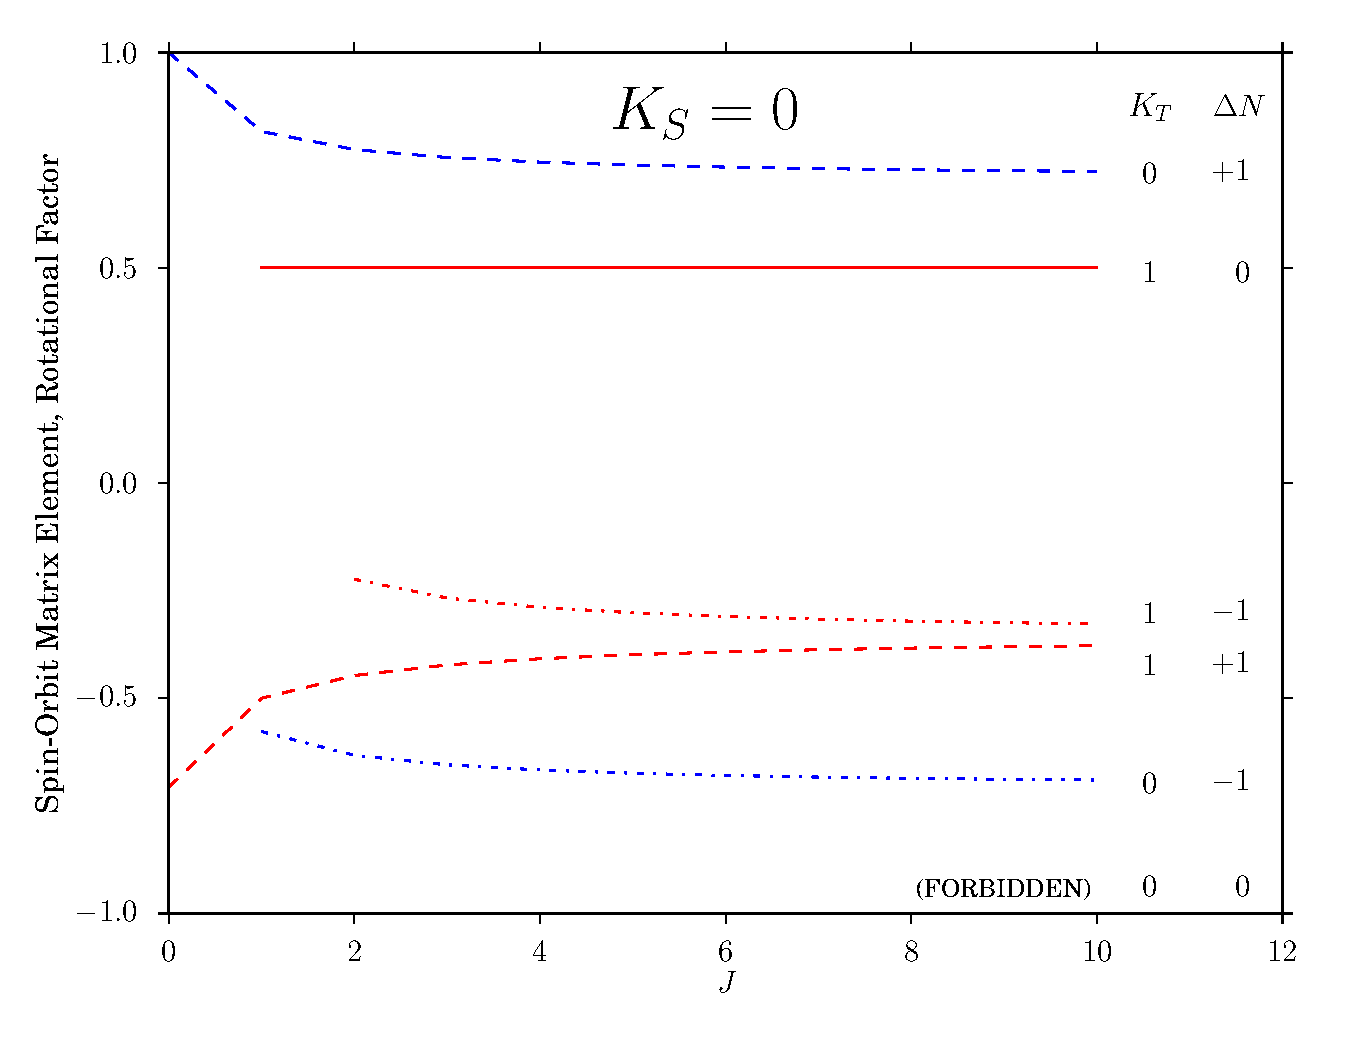
\includegraphics[width=6in]{rotational-factors-k0.pdf}
\end{figure}

%%%%%%%%%%%%%%%%%%%%%%%%%%%%%%%%%%%%%%%%%%%%%%%%%%%%%%
%%
%% END MATRIX ELEMENT FIGURE
%%
%%%%%%%%%%%%%%%%%%%%%%%%%%%%%%%%%%%%%%%%%%%%%%%%%%%%%%

The rotational selection rules between $S_1$ and $T_3$ sublevels are
perhaps best understood in terms of parity selection rules.  The
nonzero rotational factors for spin-orbit matrix elements are
illustrated on energy level diagrams in Figure \ref{fig:levels-k0} for
$K_T=0$ sublevels, and in Figure \ref{fig:levels-k1} for $K_T=1$
sublevels.  Figure \ref{fig:levels-k0} clearly illustrates that the
$3^36^1$ and $3^34^1$ $K_S=0$ sublevels may only mix with $K_T=0$
sublevels of the same vibrational symmetry.  Mixing with the $F_2$
component of a $K_T=0$ sublevel is forbidden, because the triplet
rotational level with $\Delta N=0$ has opposite parity.  Figure
\ref{fig:levels-k1} illustrates that triplet sublevels with $K_T=1$
contain levels of both parities for each value of $J$ and $N$,
therefore a level of the correct parity is always available for mixing
with a $K_S=0$ sublevel.

%%%%%%%%%%%%%%%%%%%%%%%%%%%%%%%%%%%%%%%%%%%%%%%%%%%%%%
%%
%% INSERT SINGLET-TRIPLET FIGURES HERE
%%
%%%%%%%%%%%%%%%%%%%%%%%%%%%%%%%%%%%%%%%%%%%%%%%%%%%%%%


\begin{figure}
  \caption{Diagram of spin-orbit rotational selection rules between
    the $S_1$ $3^34^1$, $3^36^1$ \Ka{0} sublevels and $T_3$ sublevels
    having $K_T=0$.  When $K_T=K_S=0$, each singlet sublevel may only
    mix with zero-order triplet sublevels of the same vibrational
    symmetry.}
  \label{fig:levels-k0}
  \centering
  \vspace{5mm}
  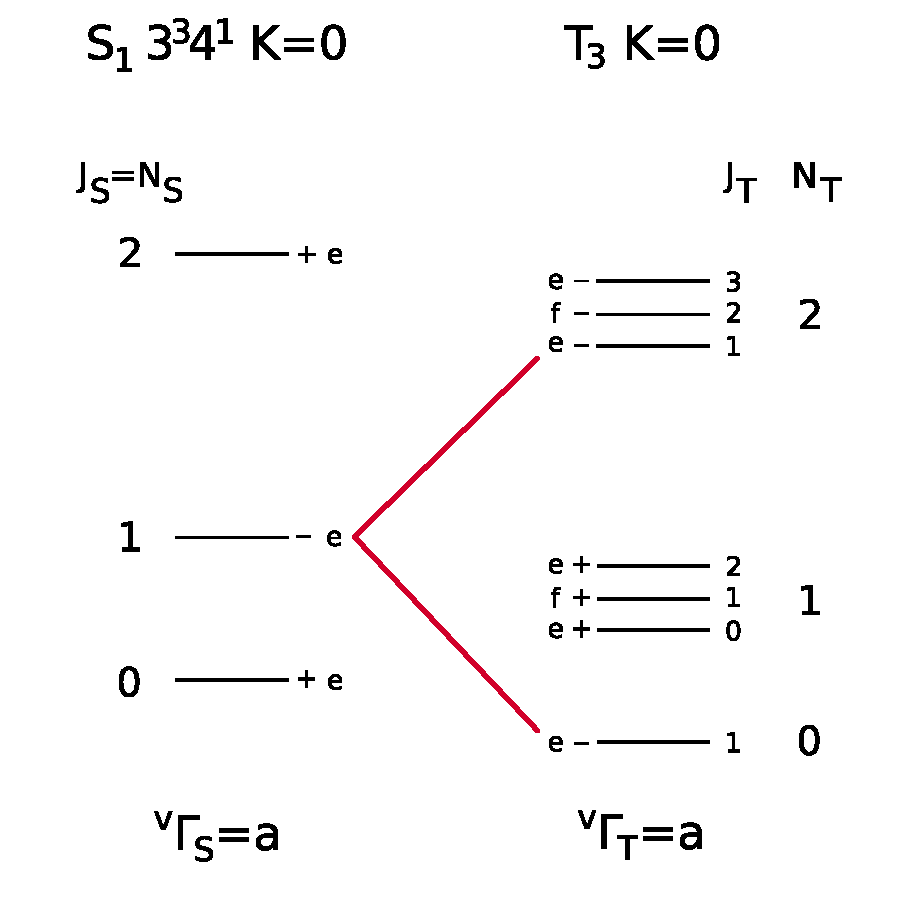
\includegraphics[width=4in,angle=90]{levels-3341}
  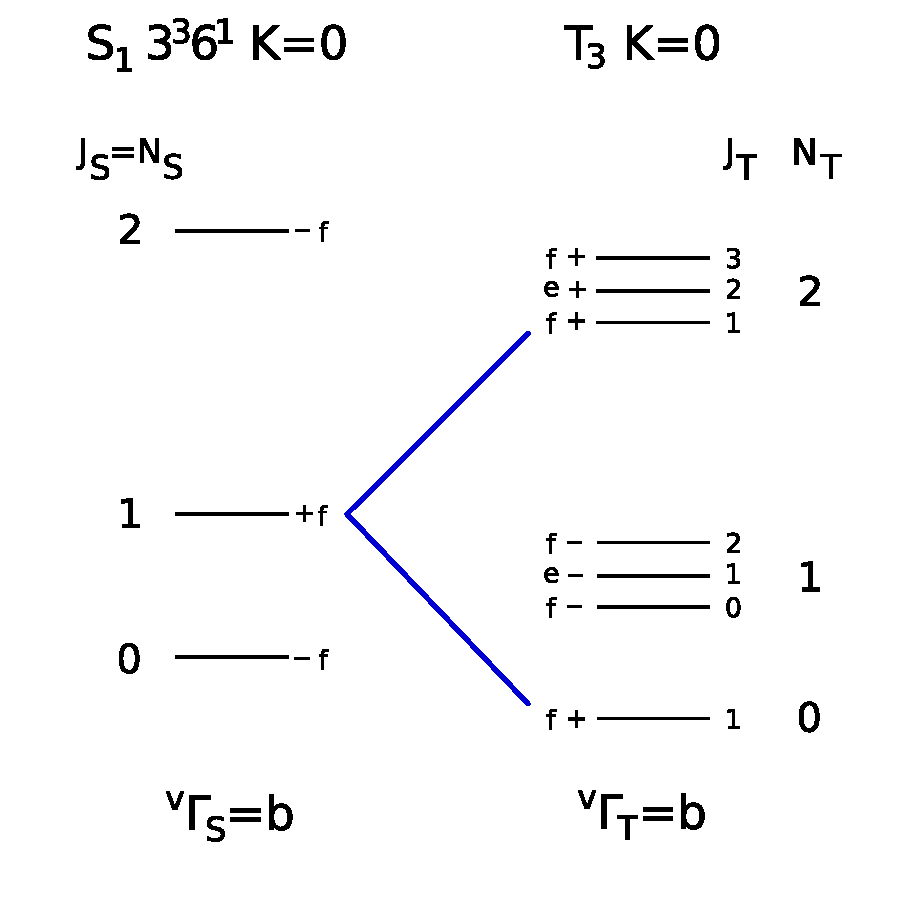
\includegraphics[width=4in,angle=90]{levels-3361}  
\end{figure}

\begin{figure}
  \caption{Diagram of spin-orbit rotational selection rules between
    the $S_1$ $3^34^1$, $3^36^1$ \Ka{0} sublevels and $T_3$ sublevels
    having $K_T=1$.  In this case, mixing is not restricted by
    vibrational symmetry, and the singlet sublevels are permitted to
    mix with the same zero-order triplet sublevel.}
  \label{fig:levels-k1}
  \centering
  \vspace{5mm}
  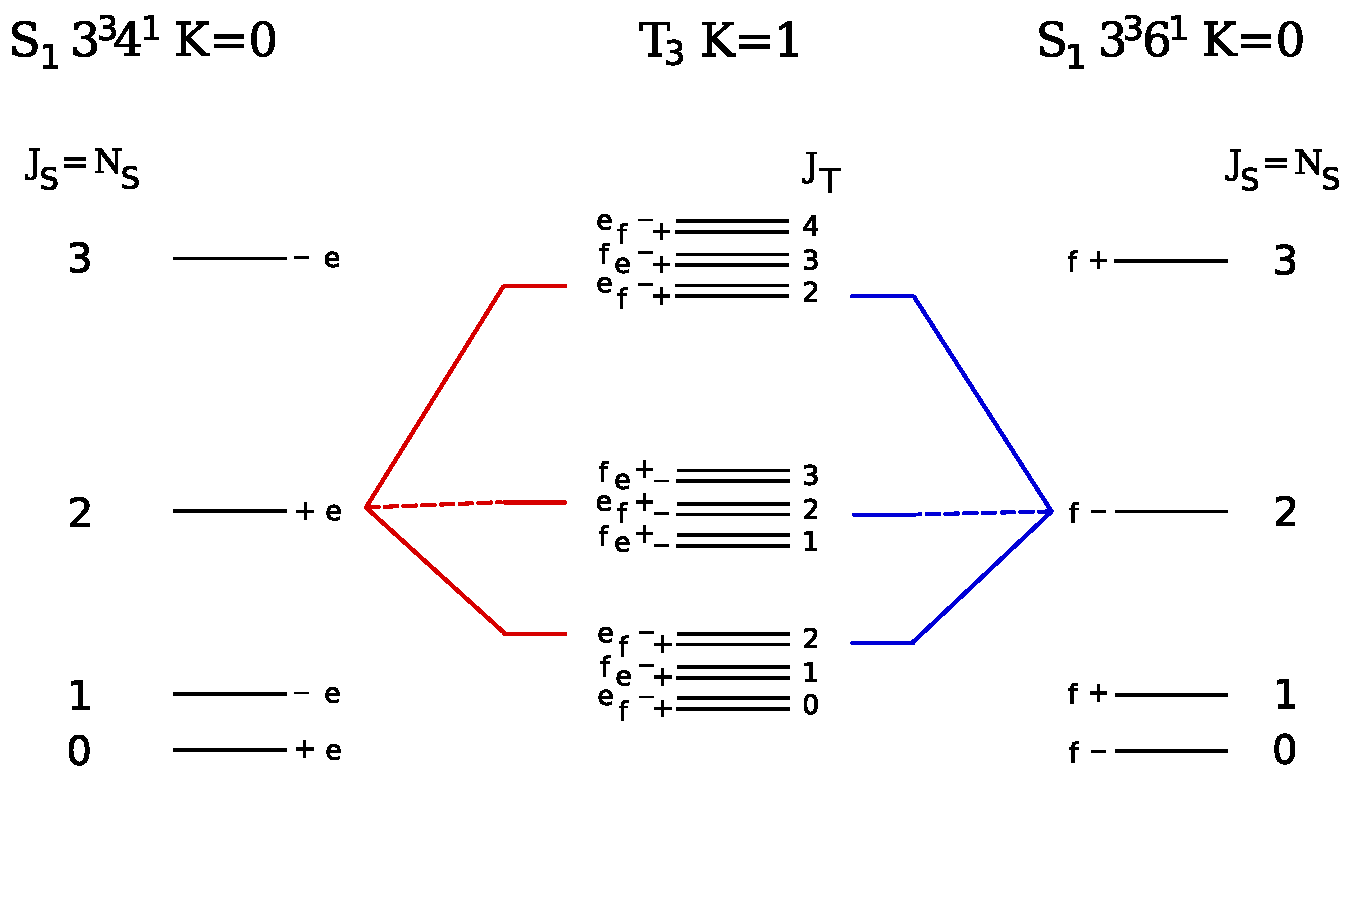
\includegraphics[width=6in,angle=90]{levels-k1}
\end{figure}

%%%%%%%%%%%%%%%%%%%%%%%%%%%%%%%%%%%%%%%%%%%%%%%%%%%%%%
%%
%% END SINGLET-TRIPLET FIGURES
%%
%%%%%%%%%%%%%%%%%%%%%%%%%%%%%%%%%%%%%%%%%%%%%%%%%%%%%%





















% \TODO{Use Bryan's program to compute overlap integrals for the two bands.}

% \TODO{Show number of modes available in each symmetry as a function
%   of energy.}



\subsection{SEELEM Spectrum: \\Characterization of the local manifold of
  $T_{1,2}$ levels}

The SSELEM spectra recorded with the individual method were fit to
Lorentzian envelopes.  To carry out the fit, the SEELEM spectrum was
first smoothed to approxiamtely twice the average line spacing, using
a Hamming window for convolution.  A Lorentzian profile was fit to the
smoothed spectrum using a non-linear least-squares regression.  Figure
\ref{fig:seelem-fits} shows the best-fit Lorentzian profiles obtained
for the $J'=1-5$ rotational levels of $3^36^1$ \Ka{0}.  The Lorentzian
half-width varies between 0.39 and 0.59 \rcm.

The full width at half maximum (FWHM) of the SEELEM distribution is
derived in Chapter 2, in terms of the $S_1 \sim T_3$ mixing angle,
$\alpha$, and the average $T_3 \sim T_{1,2}$ matrix element,
$H_{T_3T_{1,2}}$.  Our results led to the following formula:
\begin{equation}
  \text{FWHM} = 
    \frac{2}{\sqrt{e R_m}} 
    \left \lvert 
      \alpha \: H_{H_{T_3T_{1,2}}}
    \right \rvert, 
\end{equation}
where $R_m$ is a constant equal to the zero-order $S_1$ fluorescence
lifetime divided by the flight time to the SEELEM detector.  The
zero-order $S_1$ fluorescence lifetime of acetylene \astate\ is
approximately 270 ns \cite{ochi91}.  The molecular flight time from
the point of excitation to the SEELEM surface was measured as 309
\microsec\ in this study.  Evaluating this equation using the average
observed SEELEM full width at half maximum, we arrive at a value of
approximately 30 \rcm\ for the product $\alpha \times
H_{H_{T_3T_{1,2}}}$.

%%%%%%%%%%%%%%%%%%%%%%%%%%%%%%%%%%%%%%%%%%%%%%%%%%%%%%
%%
%% INSERT SEELEM FIT FIGURES
%%
%%%%%%%%%%%%%%%%%%%%%%%%%%%%%%%%%%%%%%%%%%%%%%%%%%%%%%

\begin{figure}
  \caption{Lorentzian fitting results for the $J'=1-5$ SEELEM spectra
    of the $3^36^1$ \Ka{0} sublevel.  The parameter $\Gamma$, equal to
    the half-width of the distribution, is proportional to the product
    of the $S_1 \sim T_3$ mixing angle and the average $T_3 \sim T_{1,2}$
    matrix element.  The value of $\Gamma$ is given in units of \rcm.}
  \label{fig:seelem-fits}
  \vspace{5mm}
  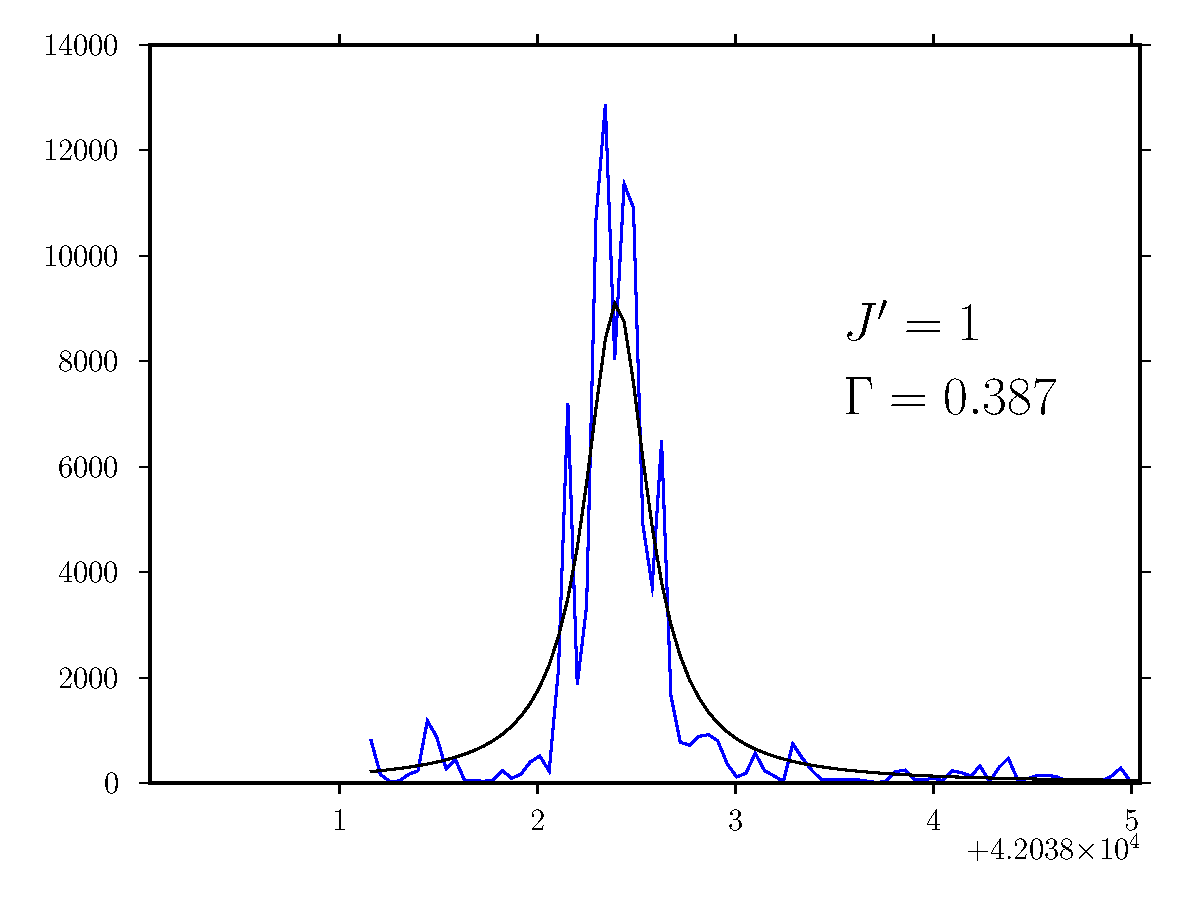
\includegraphics[width=3.2in]{3361-q1-seelemfit}
  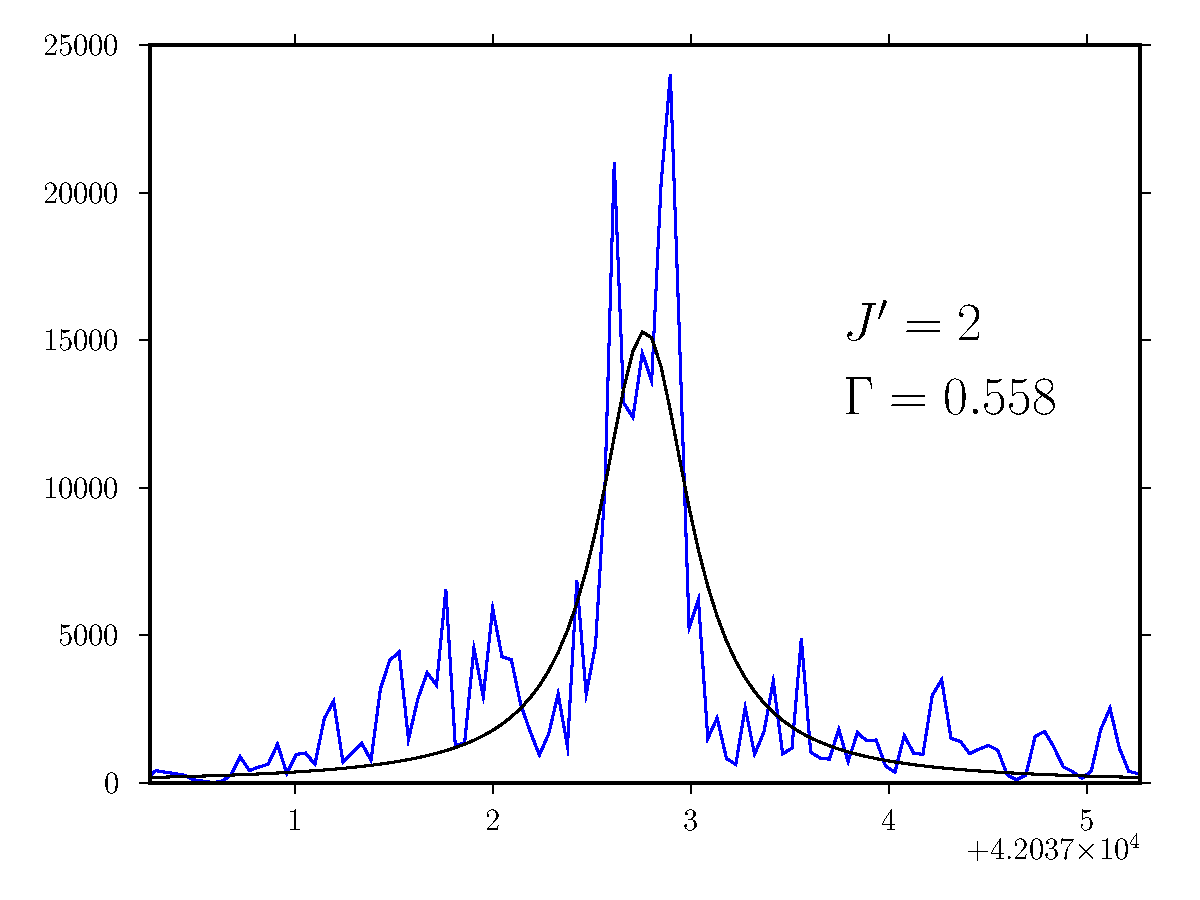
\includegraphics[width=3.2in]{3361-q2-seelemfit}
  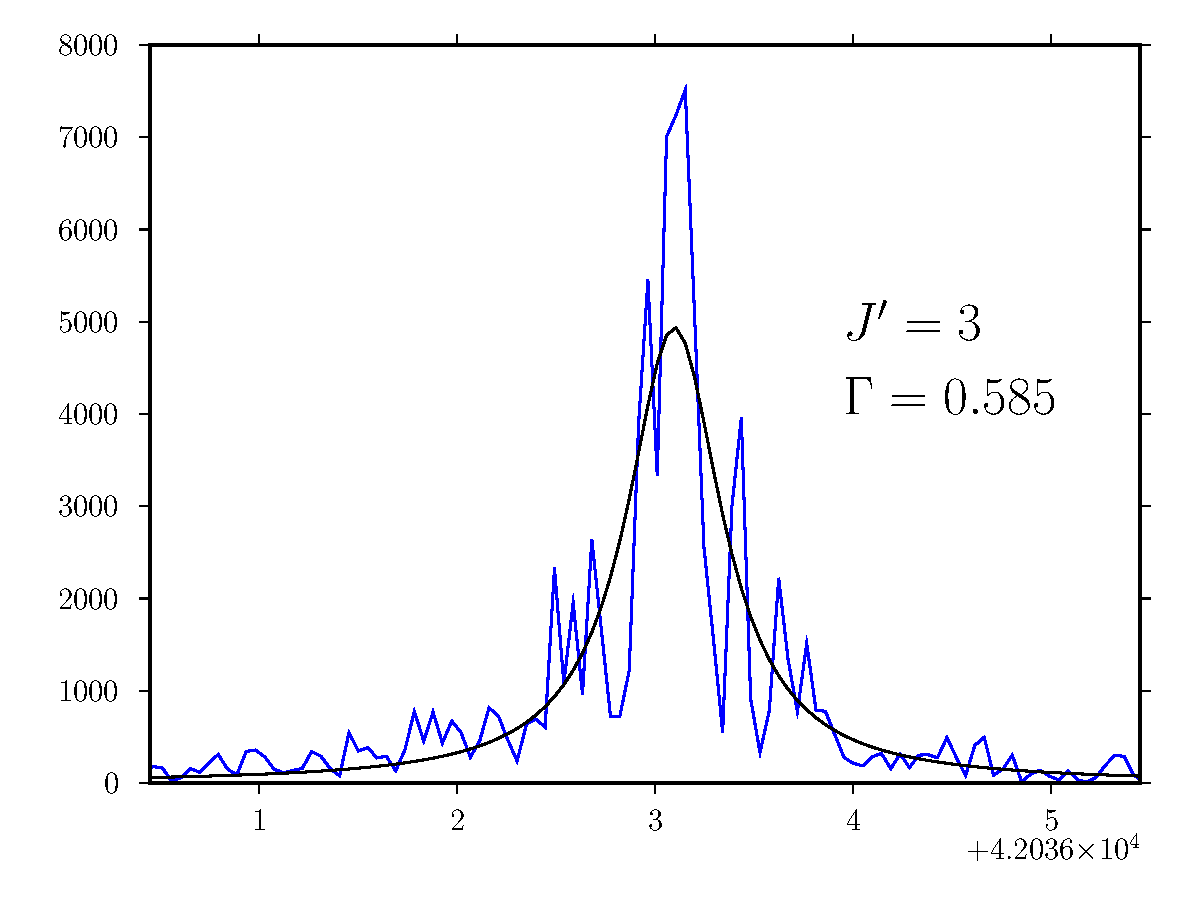
\includegraphics[width=3.2in]{3361-q3-seelemfit}
  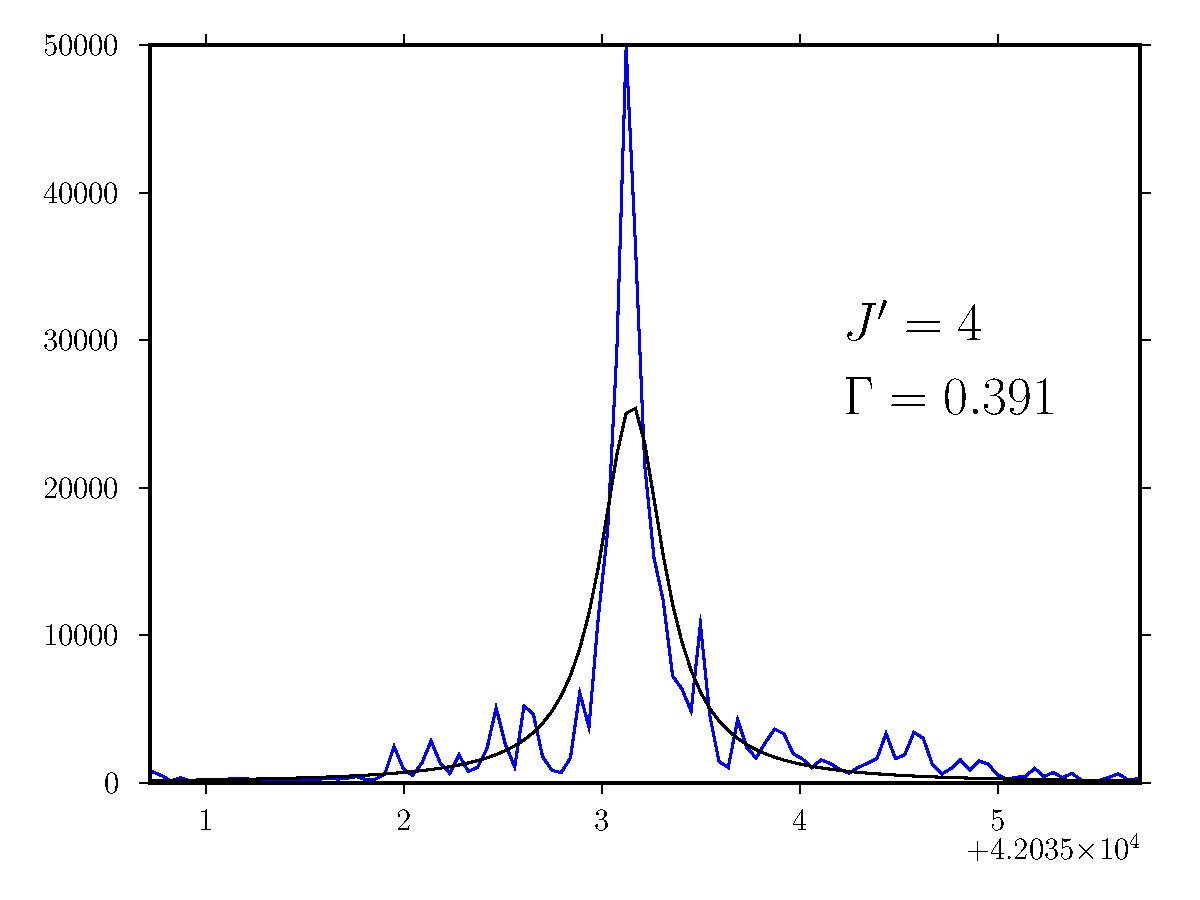
\includegraphics[width=3.2in]{3361-q4-seelemfit}
  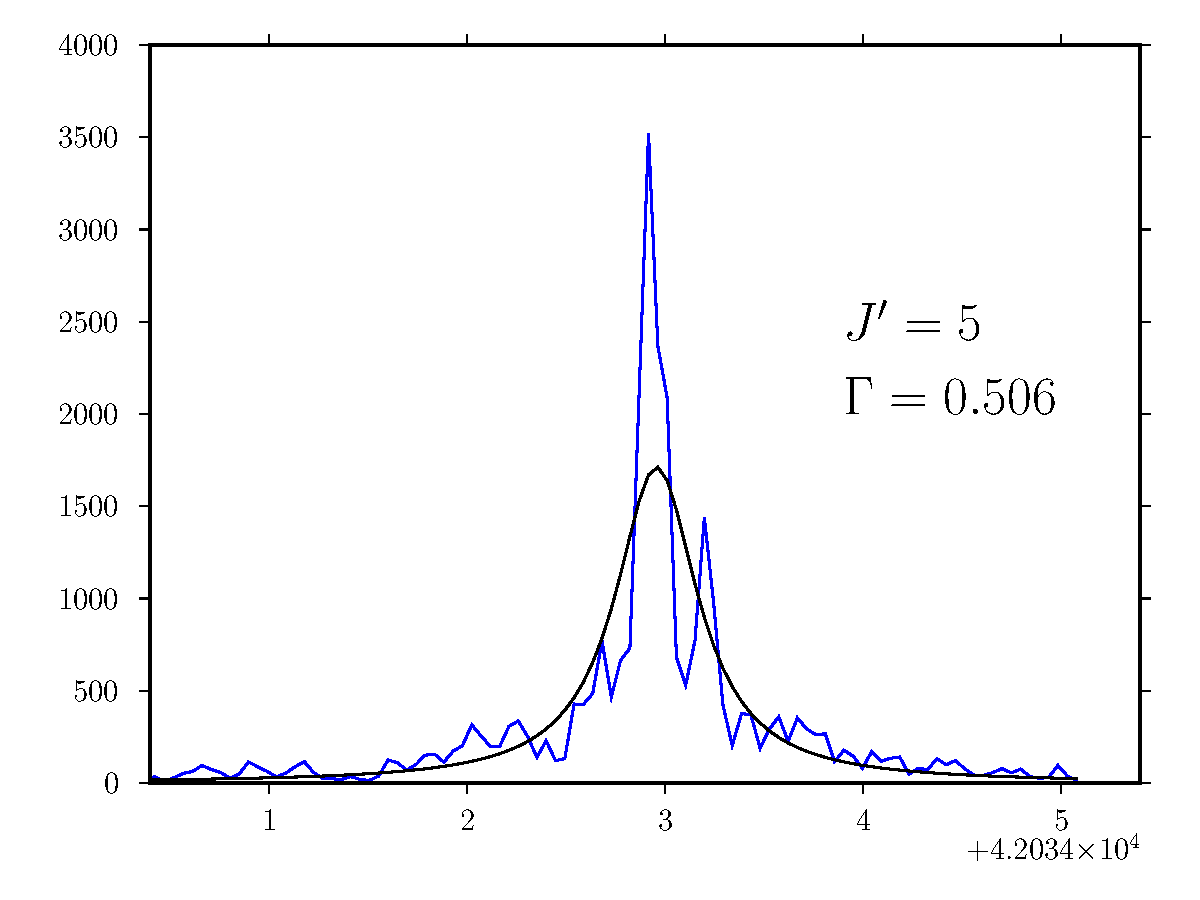
\includegraphics[width=3.2in]{3361-q5-seelemfit}
\end{figure}

%%%%%%%%%%%%%%%%%%%%%%%%%%%%%%%%%%%%%%%%%%%%%%%%%%%%%%
%%
%% END SEELEM FIT FIGURES
%%
%%%%%%%%%%%%%%%%%%%%%%%%%%%%%%%%%%%%%%%%%%%%%%%%%%%%%%

To further examine the properties of the local manifold of nominal
$T_{1,2}$ eigenstates, a reduced term value plot is prepared for the
$3^36^1$ \Ka{0} level of $S_1$ acetylene.  To construct this plot,
$S_1$ basis state rotational energies were approximately depertubed
from the spectrum by calculating the intensity-weighted center of
gravity of the LIF spectrum for

The energies of nominal triplet levels observed in the SEELEM spectrum
are shown in the plot with small markers.  For each SEELEM transition
observed in the spectrum, a horizontal bar denotes the observed SEELEM
intensity divided by the absolute energy offset from the $S_1$ level
having the same $J$.  In the limit of small fractional $S_1$
character, the width of each horizontal bar is proportional to the
spin-orbit matrix element between the SEELEM-active, nominally
$T_{1,2}$ state depicted and the $T_3$ doorway level (unobserved).
The total magnitude of the horizontal bars is normalized separately at
each value of $J'$, so comparisons are valid only between bars
appearing in the same row of the figure.  The energy spacing and
matrix elements show a remarkable uniformity, which is expected from
an extensively mixed manifold of $T_{1,2}$ levels.  The conclusions
drawn from such a figure should be treated with caution, however,
because triplet states with small matrix elements may be obscured by
others appearing with strong intensity in the SEELEM spectrum

%%%%%%%%%%%%%%%%%%%%%%%%%%%%%%%%%%%%%%%%%%%%%%%%%%%%%%
%%
%% INSERT UNFOLDED INTENSITY FIGURE
%%
%%%%%%%%%%%%%%%%%%%%%%%%%%%%%%%%%%%%%%%%%%%%%%%%%%%%%%

\begin{figure}
  \caption{Reduced term value plot for the $3^36^1$ \Ka{0} level of
    $S_1$ acetylene, showing approximately deperturbed $S_1$
    rotational energies (large markers) and the energies of nominal
    triplet levels observed in the SEELEM spectrum (small markers).
    For each SEELEM transition observed in the spectrum, a horizontal
    bar denotes the observed SEELEM intensity divided by the absolute
    energy offset from the $S_1$ level having the same $J$.  In the
    limit of small fractional $S_1$ character, the width of each
    horizontal bar is proportional to the spin-orbit matrix element
    between the SEELEM-active, nominally $T_{1,2}$ state depicted and
    the $T_3$ doorway level (unobserved).  The total magnitude of the
    horizontal bars is normalized separately at each value of $J'$, so
    comparisons are valid only between bars appearing in the same row
    of the figure.  The energy spacing and matrix elements show a
    remarkable uniformity, which is expected from an extensively mixed
    manifold of $T_{1,2}$ levels.  The conclusions drawn from such a
    figure should be treated with caution, however, because triplet
    states with small matrix elements may be obscured by others
    appearing with strong intensity in the SEELEM spectrum, as
    discussed in the text.}
  \label{fig:unfold}
  \centering
  \vspace{10mm}
  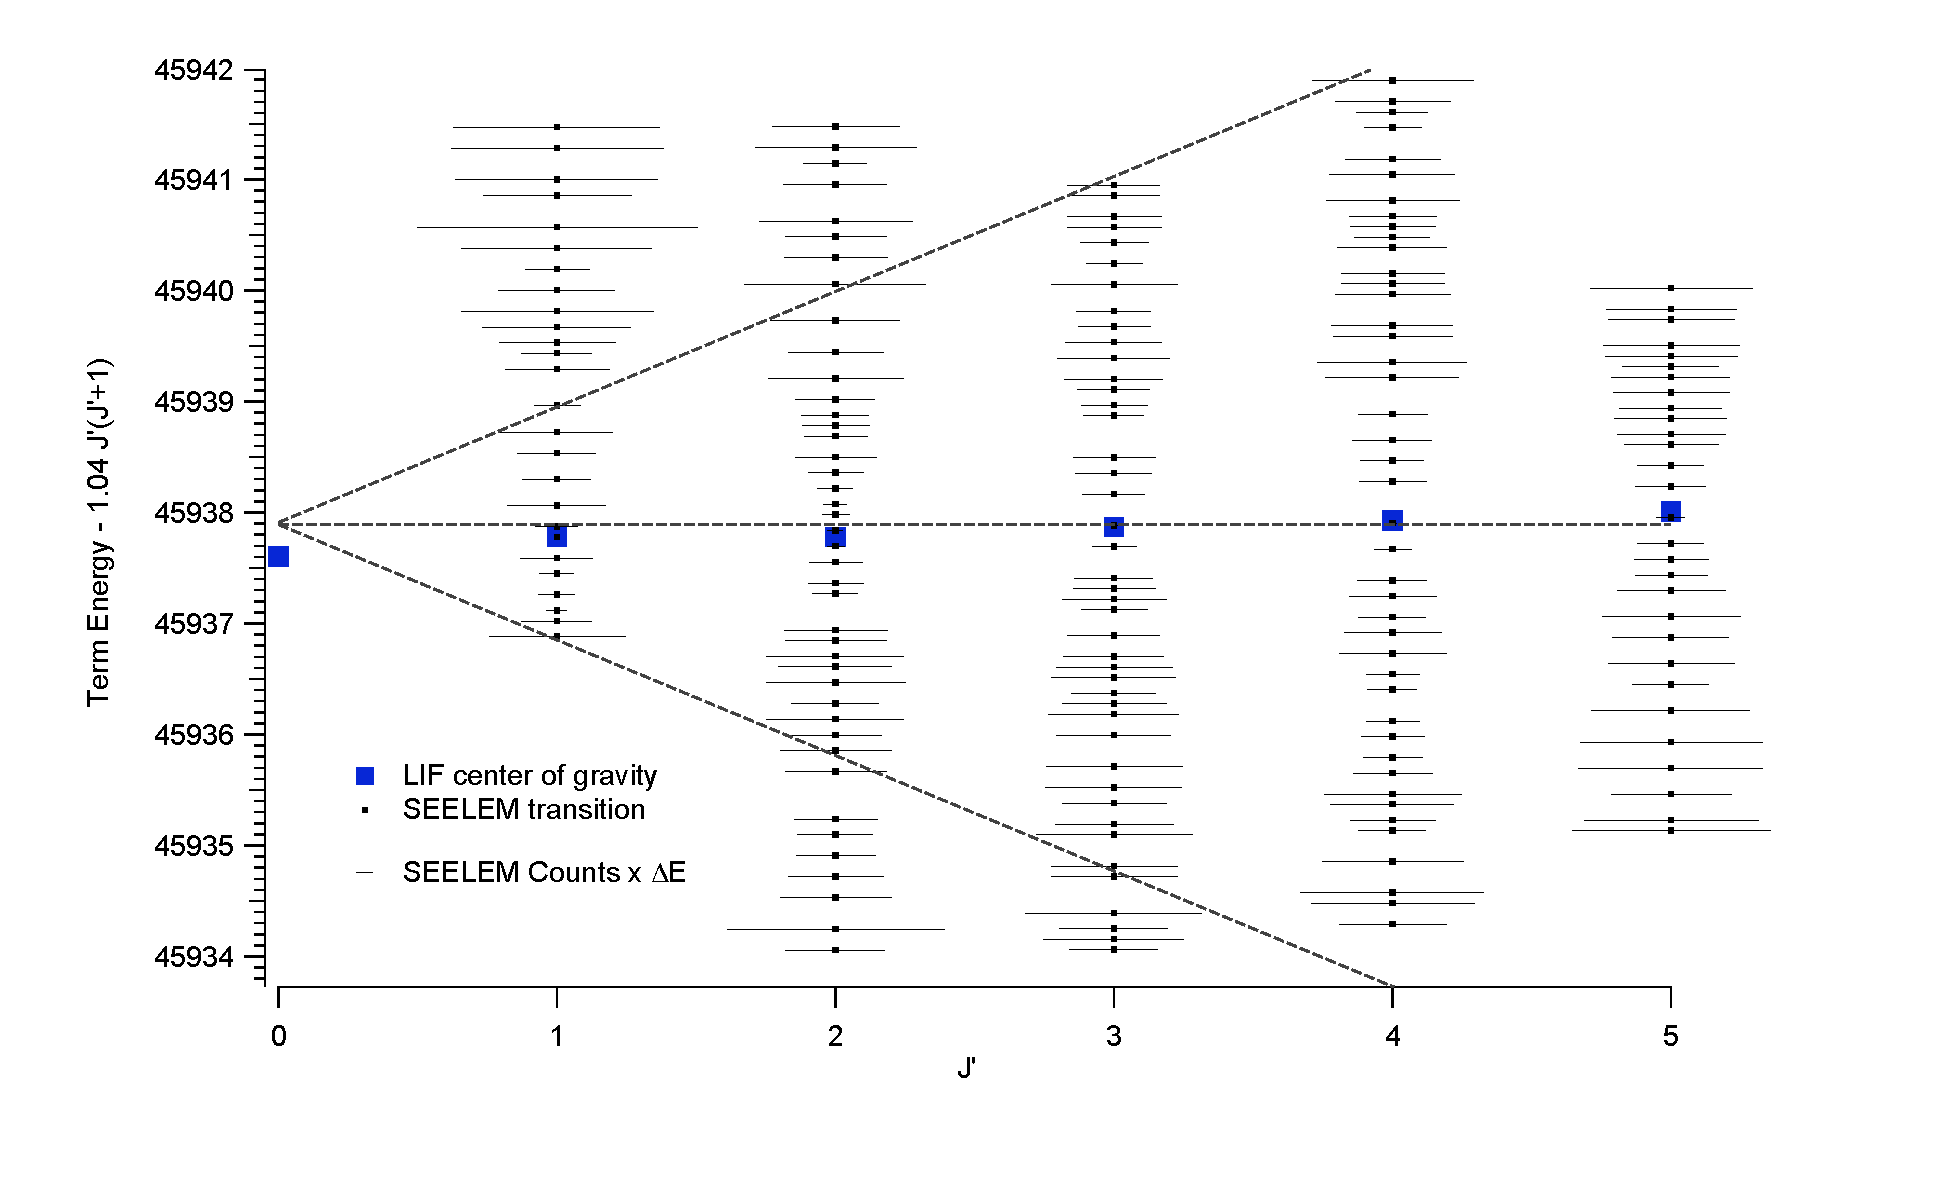
\includegraphics[width=6.2in]{redterms-3361-unfolded}
\end{figure}

%%%%%%%%%%%%%%%%%%%%%%%%%%%%%%%%%%%%%%%%%%%%%%%%%%%%%%
%%
%% END UNFOLDED INTENSITY FIGURE
%%
%%%%%%%%%%%%%%%%%%%%%%%%%%%%%%%%%%%%%%%%%%%%%%%%%%%%%%

The observation of a $J'=0$ rotational level in $3^36^1$ \Ka{0}
affords us a unique opportunity to estimate the local triplet level
density.  For a triplet vibrational sublevel having $K_T=0$ or $1$,
only a single spin component, $F_3$, is present to mix with a $J'=0$
singlet.  The vibrational symmetry of the triplet is restricted
($\Gamma_T=b$) when $K_T=0$, but unrestricted when $K_T=1$
($\Gamma_T=a$ or $b$), thus we expect to observe that the ratio of
$K_T=1$ sublevels to $K_T=0$ sublevels is 2:1.  Over an energy range
of approximately 5 \rcm, we observe approximately 26 total lines in
the SEELEM and LIF spectrum.  Of these, one must be subtracted as the
nominal $S_1$ bright state.  The 25 remaining lines are partitioned
among triplets with $K_T=0$ and $1$.  Counting only the expected
fraction of those belonging to $K_T=1$ sublevels, we are left with a
count of approximately 16.6 levels over a range of 5 \rcm, or an
observed triplet level density of $\rho_{T_{1,2}} = 3.3$ per \rcm.
The triplet level density inferred from this observation is in general
agreement with the high-resolution results of Drabbels and coworkers,
who inferred a level density of approximately 10 per \rcm from the
highly fractionated LIF spectrum of the $3^3$ \Ka{1} and $3^4$ \Ka{1}
sublevels \cite{drabbels94}.  In their observations, any of the three
spin components of a triplet sublevel with either $K_T=0, 1$ or $2$
may appear in the spectrum.  It is therefore natural that their
triplet level count should be approximately three times higher and
somewhat more uncertain than ours.






% \POINT{Present energy levels and reduced term value plot for $3^36^1$.
%   (See p.97 of 4/2007--8/2007 notebook.)} 

% \POINT{Use $\Delta_3$ statistic, $\Sigma^2$ statistic, or Fourier
%   transform methods? (See p.65 in 11/2007--1/2008 notebook.)}

\section{Discussion}

A remaining issue is: could the observed singlet$\sim$triplet mixing
in $3^34^1$ \Ka{0} be due primarily to $b$-axis Coriolis coupling with
the \Ka{1} sublevel of $3^36^1$ \Ka{1}? \TODO{Derive b-axis matrix
  element ($\approx 1.4$ \rcm) and consider energy separation between
  the $3^34^1$ \Ka{0} level and the $3^36^1$ \Ka{1} sublevel ($\approx
  42$ \rcm).  This leads to a mixing angle of about 0.03.  The
  observed splitting in $3^36^1$ \Ka{1} is approximately 1 \rcm,
  indicating what is probably a local $T_3$ perturber with a matrix
  element of 0.5 \rcm.  Mixing with $3^36^1$ \Ka{1} would lead to a
  mixing angle of approximately 0.015 with the $T_3$ perturber, which
  is not sufficient to cause 0.3 \rcm splittings in $3^34^1$ \Ka{0}.}



\TODO{Address the point of discussion: do we see too many doorways, or
  do we observe the expected number?  The answer lies in the
  definition of a doorway state -- it is simply that level of $T_3$
  with the largest mixing angle. Reiterate that we basically are
  working with a three tier model in the limit of low level density in
  the second tier.  The doorway model is a natural consequence of
  operating in this limit, because energy denominator effects make it
  likely that a single $T_3$ level mixes to a much greater degree than
  all others.  However, there is no fundamental principle which
  precludes interaction with more than one doorway.  A single doorway
  model is simply our zero-order picture.}

\TODO{Examine observations in terms of Josh's new acetylene
  wavefunction calculations.  The $\nu_3 \sim \nu_6$ anharmonic matrix
  element is much larger than the $\nu_3 \sim \nu_4$ matrix element,
  and provides a pathway for $T_{2,1} \leftarrow T_3 \leftarrow \S_1$
  coupling.  IF the stationary phase point is in a half-linear
  geometry, the combination of modes 3 and 6 is the perfect storm to
  drive a node of the vibrational wavefunction in the right direction.
  Due to the nature of the potential well, wavefunctions with
  trans-vibration alone spread out at a 45\degrees angle to the
  stationary phase point.  One node of cis-bend is enough to ``push''
  a node of the wavefunction directly toward the half-linear turning
  point. }


\TODO{Adventurous point: why have we not, to date, observe $T_3$
  doorway levels directly, in the LIF spectrum? Could it be because
  they are too fractionated into the local manifold of $T_{1,2}$
  levels?  This would reduce their fluorescence intensity greatly, and
  cause them to appear as wide Lorentzian lineshapes in the SEELEM
  spectrum.  It seems that we may be able cite our estimation of
  coupling width in this discussion.}

\section{Conclusion}

\TODO{Write this section.}

% \section{Recycle bin}

% \emph{This spring, Adam and Hans were mapping out the non-symmetric
%   bending polyads of acetylene in IR-UV double resonance experiments.
%   During this process, they encountered a number of vibrational
%   subbands with telltale signs of singlet-triplet coupling: long
%   lifetimes, fractionation, and strong quantum beats.  With help from
%   Hans, Wilton and I were able to study a few of these bands with the
%   SEELEM detector, illuminating the metastable eigenstates connected
%   to these allowed transitions.}


% Several recent \emph{ab initio} calculations have established a
% non-planar equilibrium geometry for the $T_3$ state of acetylene.  The
% most recent claculations by Bryan Wong [\emph{JCP} 126, 184307 (2007)]
% give a torsional angle of $105^\circ$, which is well in line with the
% earlier results of Ventura \emph{et al} [\emph{JCP} 118, 1702 (2003)].
% Since the $T_3$ state is known to play a role in coupling the $S_1$
% state to the bath of metastable $T_{1,2}$ states, we wish to
% investigate vibrational motions that may promote coupling between
% $S_1$ and $T_3$.  In particular, we are interested in the torsional
% mode $\nu_4'$, which twists the molecule out of a planar geometry.

% However, the two non-symmetric bending modes $\nu_4'$ and $\nu_6'$ are
% strongly coupled by Darling-Dennison and a-type Coriolis interactions.
% Our recent submission to \emph{JPC A} contains an overview of these
% effects as they relate to singlet-triplet coupling.  Anthony Merer and
% the Singlets understand these couplings very well and are now in the
% process of writing what is sure to be the classic paper on this topic.

% We wanted to ivestigate subbands where these effects are not present.

% both $K=0$ subbands show signs of strong singlet-triplet mixing.

% This particular polyad has been studied before. The most relevant
% paper is Nami and Soji's study of Zeeman quantum beats in the $3^3 B^1
% K=1$ subbands [\emph{CPL} 348, 53 (2001)].  They observe strong
% splitting and Zeeman quantum beats in the $3^3 6^1$ band, but not in
% the band involving torsion.

% Our results follow.  The first two spectra give an overview of both
% bands.  We use overlapping transitions of $J'=1-6$ in the Q-branch of
% the intermediate state to take spectra that \emph{look} like
% one-photon spectra.  Unlike Nami and Soji's observations in the $K=1$
% levels, we observe splittings and strong SEELEM signal in the $3^3
% 4^1$ band when $K=0$.

% The major advantage of working in double resonance is of course the
% ability to simplify the spectrum.  This is especially beneficial for
% SEELEM experiments, because the manifold of metastable states
% borrowing intensity from one rotational level often overlaps with that
% of the next.  We examined each rotational level in turn for $3^3 6^1$,
% collecting SEELEM data for each rotational level of the bright state
% without overlap from neighboring levels.  Since the spin-orbit
% operator is diagonal in $J$, we get this quantum number for free when
% we examine one rotational transition at a time.

% The SEELEM signals for these transitions are the strongest we have
% ever recorded for acetylene.  Even the ``weak'' intensity regions are
% full of well-resolved lines, as illustrated in a close-up of our data
% from $J'=4$.


\bibliography{master}
\bibliographystyle{plain}
\end{document}
% LocalWords:  sublevel
